\documentclass[11pt, letterpaper]{article}

% Fonts and Encoding
\usepackage[utf8]{inputenc}
\usepackage[T1]{fontenc}
\usepackage{lmodern} % High-quality Latin Modern vector font

% Math and Symbols
\usepackage{amsmath, amssymb, amsthm, amsfonts, mathrsfs, mathtools}

% Layout and Geometry
\usepackage{geometry}
\geometry{letterpaper, margin=1in}
\setlength{\parindent}{0pt}
\setlength{\parskip}{0.6em}

% Formatting and Graphics
\usepackage{graphicx, xcolor, enumitem, booktabs, array, tabularx}

% TikZ for Illustrations
\usepackage{tikz}
\usetikzlibrary{arrows.meta, positioning, shapes.geometric, calc, backgrounds, matrix}

% Clickable Links and TOC
\usepackage{hyperref}
\hypersetup{
    colorlinks=true,
    linkcolor=blue,
    filecolor=magenta,      
    urlcolor=cyan,
    pdftitle={Advanced Mathematics Topic},
}

% Theorem Environments
\newtheorem{theorem}{Theorem}[section]
\newtheorem{lemma}[theorem]{Lemma}
\newtheorem{proposition}[theorem]{Proposition}
\newtheorem{corollary}[theorem]{Corollary}
\theoremstyle{definition}
\newtheorem{definition}{Definition}[section]
\newtheorem{axiom}{Axiom}[section]
\newtheorem{example}{Example}[section]
\theoremstyle{remark}
\newtheorem{remark}{Remark}[section]

% Custom Commands (Enforced standard notation)
\newcommand{\R}{\mathbb{R}}
\newcommand{\N}{\mathbb{N}}
\newcommand{\Z}{\mathbb{Z}}
\newcommand{\Q}{\mathbb{Q}}
\newcommand{\E}{\mathbb{E}}
\newcommand{\Prob}{\mathbb{P}}
\newcommand{\F}{\mathcal{F}}

\title{\textbf{Section 7.2: Quadratic Forms} \\ \large Comprehensive Study Guide, Complete Solutions, and Advanced Modeling}
\author{Tashfeen Omran}
\date{\today}

\begin{document}

\maketitle
\tableofcontents
\newpage

% ==============================================================================
% PART 1: COMPREHENSIVE INTRODUCTION, CONTEXT, AND PREREQUISITES
% ==============================================================================
\section{Comprehensive Introduction, Context, and Prerequisites}

\subsection{Core Concepts}

Up to this point in linear algebra, nearly every equation studied has been linear in its variables, with the notable exception of the squared Euclidean norm $\|\mathbf{x}\|^2 = \mathbf{x}^T \mathbf{x} = x_1^2 + x_2^2 + \cdots + x_n^2$. A \textbf{quadratic form} generalizes this sum of squares to arbitrary homogeneous degree-two polynomials in $n$ real variables.

\begin{definition}[Quadratic Form and Its Matrix]
A \textbf{quadratic form} on $\mathbb{R}^n$ is a real-valued function $Q : \mathbb{R}^n \to \mathbb{R}$ whose value at a vector $\mathbf{x} = \begin{bmatrix} x_1 & x_2 & \cdots & x_n \end{bmatrix}^T \in \mathbb{R}^n$ can be computed by an expression of the form
\[
Q(\mathbf{x}) = \mathbf{x}^T A \mathbf{x},
\]
where $A$ is an $n \times n$ \textbf{symmetric matrix} ($A^T = A$). The matrix $A$ is called the \textbf{matrix of the quadratic form}.
\end{definition}

Expanding the matrix product $\mathbf{x}^T A \mathbf{x}$ explicitly reveals the algebraic anatomy of $Q(\mathbf{x})$:
\[
Q(\mathbf{x}) = \sum_{i=1}^n \sum_{j=1}^n a_{ij} x_i x_j = \sum_{i=1}^n a_{ii} x_i^2 + \sum_{1 \le i < j \le n} (a_{ij} + a_{ji}) x_i x_j = \sum_{i=1}^n a_{ii} x_i^2 + \sum_{1 \le i < j \le n} 2 a_{ij} x_i x_j.
\]
Two fundamental structural features emerge from this expansion:
\begin{enumerate}
    \item \textbf{Diagonal entries ($a_{ii}$):} These correspond directly to the coefficients of the pure squared terms $x_i^2$.
    \item \textbf{Off-diagonal entries ($a_{ij}$ for $i \ne j$):} Because $x_i x_j = x_j x_i$, both $a_{ij}$ and $a_{ji}$ contribute to the same \textbf{cross-product term} $x_i x_j$. Enforcing symmetry ($a_{ij} = a_{ji}$) guarantees a \emph{unique} matrix representation $A$ for any given quadratic form $Q(\mathbf{x})$: the coefficient of $x_i x_j$ ($i \ne j$) in $Q(\mathbf{x})$ is split evenly between the $(i,j)$- and $(j,i)$-entries of $A$.
\end{enumerate}

When $A$ is a diagonal matrix, all off-diagonal entries vanish, and $Q(\mathbf{x}) = \lambda_1 x_1^2 + \lambda_2 x_2^2 + \cdots + \lambda_n x_n^2$ contains \emph{no cross-product terms}. Diagonal quadratic forms are dramatically simpler to evaluate, graph, and bound. Remarkably, by changing coordinates via an orthogonal matrix, \emph{every} quadratic form can be converted into one with no cross-product terms.

\begin{definition}[Definiteness Classification of Quadratic Forms]
A quadratic form $Q(\mathbf{x}) = \mathbf{x}^T A \mathbf{x}$ on $\mathbb{R}^n$ (and correspondingly, its symmetric matrix $A$) is classified as:
\begin{itemize}
    \item \textbf{Positive definite} if $Q(\mathbf{x}) > 0$ for all $\mathbf{x} \ne \mathbf{0}$ in $\mathbb{R}^n$.
    \item \textbf{Negative definite} if $Q(\mathbf{x}) < 0$ for all $\mathbf{x} \ne \mathbf{0}$ in $\mathbb{R}^n$.
    \item \textbf{Indefinite} if $Q(\mathbf{x})$ assumes both strictly positive and strictly negative values on $\mathbb{R}^n$.
    \item \textbf{Positive semidefinite} if $Q(\mathbf{x}) \ge 0$ for all $\mathbf{x} \in \mathbb{R}^n$.
    \item \textbf{Negative semidefinite} if $Q(\mathbf{x}) \le 0$ for all $\mathbf{x} \in \mathbb{R}^n$.
\end{itemize}
\end{definition}

\subsection{Intuition and Derivation}

Why can we always eliminate cross-product terms, and why do eigenvalues govern the sign of $Q(\mathbf{x})$? The explanation rests on combining a linear \textbf{change of variable} with the Spectral Theorem for symmetric matrices (Section 7.1).

Suppose we introduce a new coordinate vector $\mathbf{y} \in \mathbb{R}^n$ related to $\mathbf{x}$ by an invertible matrix $P$:
\[
\mathbf{x} = P\mathbf{y}, \qquad \text{or equivalently,} \qquad \mathbf{y} = P^{-1}\mathbf{x}.
\]
Substituting $\mathbf{x} = P\mathbf{y}$ into $Q(\mathbf{x}) = \mathbf{x}^T A \mathbf{x}$ and applying the transpose rule $(P\mathbf{y})^T = \mathbf{y}^T P^T$ gives:
\[
\mathbf{x}^T A \mathbf{x} = (P\mathbf{y})^T A (P\mathbf{y}) = \mathbf{y}^T P^T A P \mathbf{y} = \mathbf{y}^T (P^T A P) \mathbf{y}.
\]
Notice that the new matrix of the quadratic form in $\mathbf{y}$-coordinates is $P^T A P$, which is a \emph{congruence transformation} of $A$, not a similarity transformation $P^{-1} A P$—unless $P^T = P^{-1}$, i.e., unless $P$ is an \textbf{orthogonal matrix}.

Because $A$ is symmetric, the Spectral Theorem guarantees the existence of an orthogonal matrix $P = \begin{bmatrix} \mathbf{u}_1 & \mathbf{u}_2 & \cdots & \mathbf{u}_n \end{bmatrix}$ whose columns are orthonormal eigenvectors of $A$, such that
\[
P^T A P = P^{-1} A P = D = \operatorname{diag}(\lambda_1, \lambda_2, \dots, \lambda_n),
\]
where $\lambda_1, \dots, \lambda_n$ are the real eigenvalues of $A$. Under this orthogonal change of variable $\mathbf{x} = P\mathbf{y}$, the quadratic form collapses cleanly into a pure sum of weighted squares:
\[
Q(\mathbf{x}) = \mathbf{x}^T A \mathbf{x} = \mathbf{y}^T D \mathbf{y} = \lambda_1 y_1^2 + \lambda_2 y_2^2 + \cdots + \lambda_n y_n^2.
\]
This derivation directly proves the \textbf{Principal Axes Theorem} (Theorem 4): the orthonormal eigenvectors $\mathbf{u}_1, \dots, \mathbf{u}_n$ form the \textbf{principal axes} of the quadratic form. Geometrically, an orthogonal change of variable $\mathbf{x} = P\mathbf{y}$ rotates (and possibly reflects) the coordinate axes so that the level curve or surface $\mathbf{x}^T A \mathbf{x} = c$ aligns in standard position with the new axes $y_1, \dots, y_n$.

\begin{figure}[htbp]
\centering
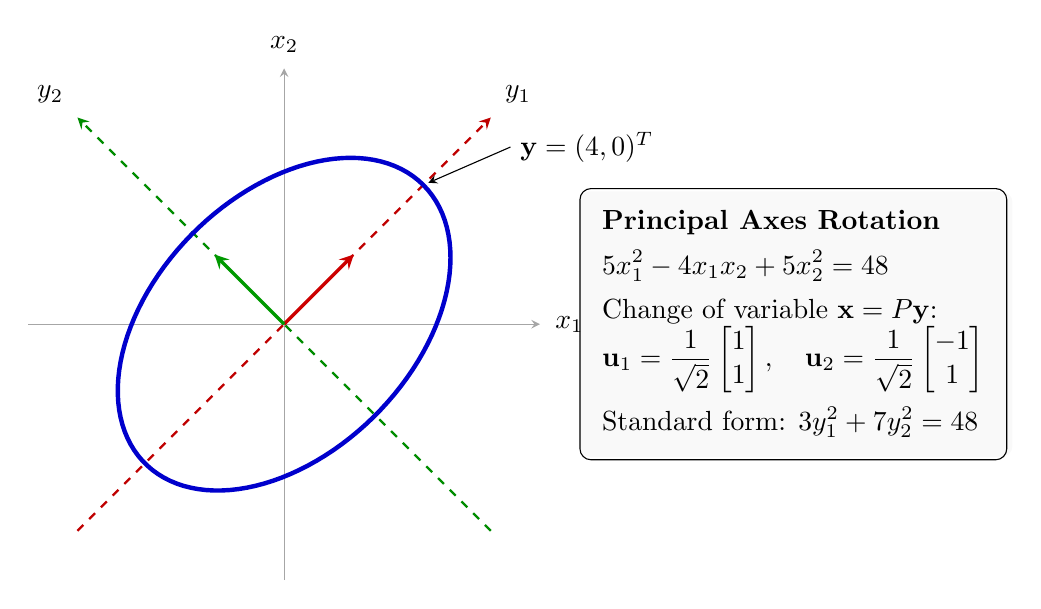
\begin{tikzpicture}[scale=1.25]
    % Layer 1: Background fill for legend
    \fill[gray!5, rounded corners=4pt] (3.0, -1.35) rectangle (7.4, 1.35);

    % Layer 2: Grid and Coordinate Axes
    \draw[->, >=stealth, thin, gray!70] (-2.6, 0) -- (2.6, 0) node[right=2pt, black] {$x_1$};
    \draw[->, >=stealth, thin, gray!70] (0, -2.6) -- (0, 2.6) node[above=2pt, black] {$x_2$};

    % Rotated Principal Axes (y1, y2 at 45 degrees)
    \draw[->, >=stealth, thick, red!75!black, dashed] (-2.1, -2.1) -- (2.1, 2.1) node[above right=2pt, black] {$y_1$};
    \draw[->, >=stealth, thick, green!55!black, dashed] (2.1, -2.1) -- (-2.1, 2.1) node[above left=2pt, black] {$y_2$};

    % Layer 3: Primary Plot - Ellipse 5x_1^2 - 4x_1x_2 + 5x_2^2 = 48 (scaled by 0.5)
    % y1 = 4 cos(t), y2 = sqrt(48/7) sin(t) ~ 2.6186 sin(t)
    % x1 = 0.5*(y1 - y2)/sqrt(2), x2 = 0.5*(y1 + y2)/sqrt(2)
    \draw[ultra thick, blue!80!black] plot[domain=0:360, samples=120]
        ({0.5*0.7071*(4*cos(\x) - 2.6186*sin(\x))}, {0.5*0.7071*(4*cos(\x) + 2.6186*sin(\x))});

    % Eigenvector unit markers (scaled for visibility)
    \draw[->, >=stealth, very thick, red!80!black] (0,0) -- (0.7071, 0.7071);
    \draw[->, >=stealth, very thick, green!60!black] (0,0) -- (-0.7071, 0.7071);

    % Layer 4: Off-axis Callout and Legend
    \draw[->, >=stealth, thin, black, shorten >=2pt] (2.3, 1.8) -- (1.414, 1.414);
    \node[black, anchor=west] at (2.3, 1.8) {$\mathbf{y} = (4, 0)^T$};

    \node[draw=gray!60, rounded corners=4pt, align=left, inner sep=8pt, anchor=west, black] at (3.0, 0) {
        \textbf{Principal Axes Rotation} \\[4pt]
        $\displaystyle 5x_1^2 - 4x_1x_2 + 5x_2^2 = 48$ \\[4pt]
        Change of variable $\mathbf{x} = P\mathbf{y}$: \\
        $\displaystyle \mathbf{u}_1 = \frac{1}{\sqrt{2}}\begin{bmatrix} 1 \\ 1 \end{bmatrix}, \quad \mathbf{u}_2 = \frac{1}{\sqrt{2}}\begin{bmatrix} -1 \\ 1 \end{bmatrix}$ \\[4pt]
        Standard form: $\displaystyle 3y_1^2 + 7y_2^2 = 48$
    };
\end{tikzpicture}
\caption{Geometric view of the Principal Axes Theorem for Example 5 ($5x_1^2 - 4x_1x_2 + 5x_2^2 = 48$). Rotating the $(x_1, x_2)$-axes by $45^\circ$ into the $(y_1, y_2)$-axes aligns the ellipse into standard position.}
\end{figure}

Furthermore, because $P$ is invertible, $\mathbf{x} \ne \mathbf{0}$ if and only if $\mathbf{y} \ne \mathbf{0}$. Looking at the diagonalized form
\[
Q(\mathbf{x}) = \lambda_1 y_1^2 + \lambda_2 y_2^2 + \cdots + \lambda_n y_n^2,
\]
every $y_i^2 \ge 0$, and at least one $y_i^2 > 0$ whenever $\mathbf{x} \ne \mathbf{0}$. Consequently, the sign of $Q(\mathbf{x})$ across all $\mathbf{x} \ne \mathbf{0}$ is completely controlled by the signs of the eigenvalues $\lambda_1, \dots, \lambda_n$: if all $\lambda_i > 0$, then $Q(\mathbf{x}) > 0$; if all $\lambda_i < 0$, then $Q(\mathbf{x}) < 0$; and if some $\lambda_i > 0$ while some $\lambda_j < 0$, then setting $\mathbf{y} = \mathbf{e}_i$ yields $Q(\mathbf{x}) = \lambda_i > 0$ while $\mathbf{y} = \mathbf{e}_j$ yields $Q(\mathbf{x}) = \lambda_j < 0$, proving $Q$ is indefinite.

\begin{figure}[htbp]
\centering
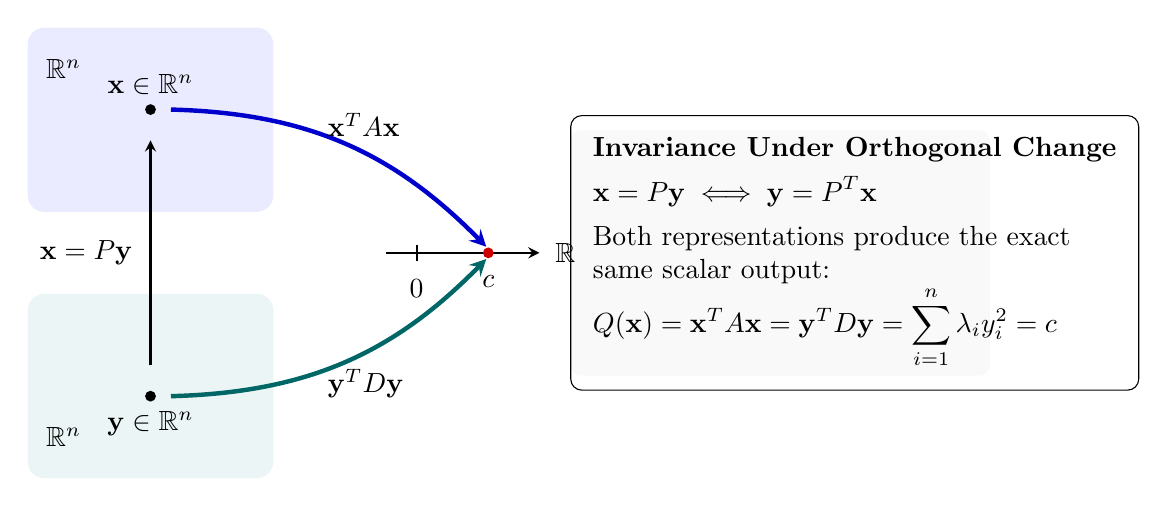
\begin{tikzpicture}[scale=1.3]
    % Layer 1: Background regions for the two vector spaces
    \fill[blue!8, rounded corners=6pt] (-2.2, 0.4) rectangle (0.2, 2.2);
    \fill[teal!8, rounded corners=6pt] (-2.2, -2.2) rectangle (0.2, -0.4);
    \fill[gray!5, rounded corners=4pt] (3.1, -1.2) rectangle (7.2, 1.2);

    % Layer 2: Real number line on the right
    \draw[->, >=stealth, thick, black] (1.3, 0) -- (2.8, 0) node[right=2pt, black] {$\mathbb{R}$};
    \draw[thick, black] (1.6, 0.08) -- (1.6, -0.08) node[below=3pt, black] {$0$};
    \fill[red!80!black] (2.3, 0) circle (1.5pt);
    \node[below=3pt, black] at (2.3, -0.05) {$c$};

    % Layer 3: Points and mappings
    \fill[black] (-1.0, 1.4) circle (1.5pt);
    \node[above=2pt, black] at (-1.0, 1.4) {$\mathbf{x} \in \mathbb{R}^n$};

    \fill[black] (-1.0, -1.4) circle (1.5pt);
    \node[below=2pt, black] at (-1.0, -1.4) {$\mathbf{y} \in \mathbb{R}^n$};

    % Vertical mapping P
    \draw[->, >=stealth, thick, black] (-1.0, -1.1) -- (-1.0, 1.1);
    \node[left=3pt, black] at (-1.0, 0) {$\mathbf{x} = P\mathbf{y}$};

    % Curved quadratic form arrows
    \draw[->, >=stealth, ultra thick, blue!80!black] (-0.8, 1.4) to[bend left=22] (2.28, 0.06);
    \draw[->, >=stealth, ultra thick, teal!80!black] (-0.8, -1.4) to[bend right=22] (2.28, -0.06);

    % Layer 4: Labels and Single-Node Annotation
    \node[above right=2pt, black] at (0.6, 1.0) {$\mathbf{x}^T A \mathbf{x}$};
    \node[below right=2pt, black] at (0.6, -1.0) {$\mathbf{y}^T D \mathbf{y}$};
    \node[left=3pt, black] at (-1.5, 1.8) {$\mathbb{R}^n$};
    \node[left=3pt, black] at (-1.5, -1.8) {$\mathbb{R}^n$};

    \node[draw=gray!60, rounded corners=4pt, align=left, inner sep=8pt, anchor=west, black] at (3.1, 0) {
        \textbf{Invariance Under Orthogonal Change} \\[4pt]
        $\displaystyle \mathbf{x} = P\mathbf{y} \iff \mathbf{y} = P^T \mathbf{x}$ \\[4pt]
        Both representations produce the exact \\
        same scalar output: \\
        $\displaystyle Q(\mathbf{x}) = \mathbf{x}^T A \mathbf{x} = \mathbf{y}^T D \mathbf{y} = \sum_{i=1}^n \lambda_i y_i^2 = c$
    };
\end{tikzpicture}
\caption{Schematic of the change of variable $\mathbf{x} = P\mathbf{y}$ showing invariance of the quadratic form value.}
\end{figure}

\subsection{Historical Context and Motivation}

The study of quadratic forms originated in 18th-century celestial mechanics, geometry, and number theory. Astronomers and physicists such as Leonhard Euler, Joseph-Louis Lagrange, and Pierre-Simon Laplace encountered quadratic expressions when classifying planetary orbits (conic sections rotated away from coordinate axes), studying moments of inertia of rigid rotating bodies, and analyzing small oscillations around equilibrium via kinetic and potential energy. Specifically, finding the "principal axes of inertia" of a rigid body or reducing a rotated conic $ax_1^2 + 2bx_1x_2 + dx_2^2 = c$ to standard form directly motivated the Principal Axes Theorem.

Simultaneously, in pure mathematics, Carl Friedrich Gauss systematically investigated binary quadratic forms $ax^2 + 2bxy + cy^2$ with integer coefficients in his landmark \emph{Disquisitiones Arithmeticae} (1801) to determine which integers can be represented by such forms. Later in the 19th century, Augustin-Louis Cauchy, Karl Weierstrass, and James Joseph Sylvester formalized the spectral theory of symmetric matrices and inertia, transforming quadratic forms into a foundational tool of multivariable optimization (via the Hessian matrix), differential geometry (the first and second fundamental forms for surface curvature), and modern statistics (variance-covariance ellipsoids).

\subsection{Key Formulas}

\renewcommand{\arraystretch}{1.5}
\begin{tabularx}{\textwidth}{>{$\displaystyle}l<{$} >{$\displaystyle}l<{$} X}
\toprule
\textbf{Concept} & \textbf{Formula} & \textbf{Description / Notes} \\
\midrule
\text{Quadratic Form} & Q(\mathbf{x}) = \mathbf{x}^T A \mathbf{x} & $A$ is an $n \times n$ symmetric matrix ($A^T = A$). \\
\addlinespace[4pt]
\text{Matrix Extraction} & a_{ii} = \text{coeff}(x_i^2), \quad a_{ij} = a_{ji} = \frac{1}{2}\text{coeff}(x_i x_j) & Split each cross-product coefficient evenly for $i \ne j$. \\
\addlinespace[4pt]
\text{Change of Variable} & \mathbf{x} = P\mathbf{y}, \qquad \mathbf{x}^T A \mathbf{x} = \mathbf{y}^T (P^T A P) \mathbf{y} & New matrix is $P^T A P$; if $P$ is orthogonal, $P^T = P^{-1}$. \\
\addlinespace[4pt]
\text{Principal Axes Form} & \mathbf{x}^T A \mathbf{x} = \mathbf{y}^T D \mathbf{y} = \sum_{i=1}^n \lambda_i y_i^2 & Columns of $P$ are orthonormal eigenvectors of $A$. \\
\addlinespace[4pt]
\text{Coordinate Recovery} & \mathbf{y} = P^T \mathbf{x} & Expresses $\mathbf{x}$ in the principal axes basis when $P$ is orthogonal. \\
\addlinespace[4pt]
2 \times 2 \text{ Trace \& Det} & \lambda_1 + \lambda_2 = a + d, \qquad \lambda_1 \lambda_2 = ad - b^2 & Fast classification for $A = \begin{bmatrix} a & b \\ b & d \end{bmatrix}$ without eigenvalues. \\
\addlinespace[4pt]
\text{Cholesky Factorization} & A = R^T R & Exists iff $A$ is positive definite ($R$ upper triangular, $r_{ii} > 0$). \\
\bottomrule
\end{tabularx}

\subsection{Prerequisites}

To master Section 7.2, the following foundational skills are essential:
\begin{itemize}
    \item \textbf{Matrix Algebra and Transposes:} Fluency with matrix-vector multiplication, matrix transposition $(AB)^T = B^T A^T$, and recognizing symmetric matrices ($A^T = A$).
    \item \textbf{Eigenvalues and Eigenvectors (Chapter 5):} Computing the characteristic polynomial $\det(A - \lambda I) = 0$, solving quadratic and factored higher-degree polynomials, and finding a basis for each eigenspace $\operatorname{Nul}(A - \lambda I)$.
    \item \textbf{Orthogonality and Gram-Schmidt (Chapter 6):} Computing dot products $\mathbf{u} \cdot \mathbf{v} = \mathbf{u}^T \mathbf{v}$, normalizing vectors ($\mathbf{u} = \mathbf{v}/\|\mathbf{v}\|$), recognizing orthogonal matrices ($P^T P = I \iff P^{-1} = P^T$), and applying the Gram-Schmidt process to orthogonalize bases within multi-dimensional eigenspaces.
    \item \textbf{Orthogonal Diagonalization (Section 7.1):} Knowing that symmetric matrices have real eigenvalues, eigenvectors from distinct eigenspaces are automatically orthogonal, and $A = P D P^T$ for every symmetric matrix $A$.
    \item \textbf{Change of Basis (Section 4.4):} Understanding $\mathbf{x} = P\mathbf{y}$ as converting a coordinate vector $\mathbf{y}$ relative to the basis formed by the columns of $P$ into standard coordinates $\mathbf{x}$.
\end{itemize}

\newpage

% ==============================================================================
% PART 2: DETAILED HOMEWORK SOLUTIONS
% ==============================================================================
\section{Detailed Homework Solutions}

Below are complete, step-by-step solutions to every exercise in Section 7.2 (Exercises 1--36) from the assigned text, as well as the Section 7.2 Practice Problem for completeness.

\subsection*{Practice Problem (Page 454)}
\textbf{Original Problem:} Describe a positive semidefinite matrix $A$ in terms of its eigenvalues.

\textbf{Solution:}
Let $A$ be an $n \times n$ symmetric matrix. By the Principal Axes Theorem (Theorem 4), there exists an orthogonal change of variable $\mathbf{x} = P\mathbf{y}$ (with $P$ orthogonal, so $P^T A P = D$) such that
\[
\mathbf{x}^T A \mathbf{x} = \mathbf{y}^T D \mathbf{y} = \lambda_1 y_1^2 + \lambda_2 y_2^2 + \cdots + \lambda_n y_n^2,
\]
where $\lambda_1, \dots, \lambda_n$ are the eigenvalues of $A$.
\begin{itemize}
    \item \emph{($\Longrightarrow$)} Suppose $A$ is positive semidefinite, so $\mathbf{x}^T A \mathbf{x} \ge 0$ for all $\mathbf{x} \in \mathbb{R}^n$. If any eigenvalue $\lambda_i$ were strictly negative, then choosing $\mathbf{y} = \mathbf{e}_i$ (the $i$-th standard basis vector) and $\mathbf{x} = P\mathbf{e}_i$ would yield $\mathbf{x}^T A \mathbf{x} = \lambda_i (1)^2 = \lambda_i < 0$, a contradiction. Thus, every eigenvalue of $A$ must satisfy $\lambda_i \ge 0$.
    \item \emph{($\Longleftarrow$)} Conversely, if $\lambda_i \ge 0$ for all $i = 1, \dots, n$, then since $y_i^2 \ge 0$ for all $\mathbf{y} \in \mathbb{R}^n$, we have $\mathbf{x}^T A \mathbf{x} = \sum_{i=1}^n \lambda_i y_i^2 \ge 0$ for all $\mathbf{x} \in \mathbb{R}^n$.
\end{itemize}
\textbf{Final Answer:} A symmetric matrix $A$ is positive semidefinite if and only if all of its eigenvalues are nonnegative ($\lambda_i \ge 0$ for all $i$).

\hrulefill

\subsection*{Exercise 1}
\textbf{Original Problem:} Compute the quadratic form $\mathbf{x}^T A \mathbf{x}$, when $A = \begin{bmatrix} 3 & 1/4 \\ 1/4 & 1 \end{bmatrix}$ and:
\begin{enumerate}[label=\alph*.]
    \item $\mathbf{x} = \begin{bmatrix} x_1 \\ x_2 \end{bmatrix}$
    \item $\mathbf{x} = \begin{bmatrix} 8 \\ 1 \end{bmatrix}$
    \item $\mathbf{x} = \begin{bmatrix} 1 \\ 4 \end{bmatrix}$
\end{enumerate}

\textbf{Solution:}
\begin{enumerate}[label=\alph*.]
    \item First compute $A\mathbf{x}$, then multiply on the left by $\mathbf{x}^T$:
    \begin{align*}
    \mathbf{x}^T A \mathbf{x} &= \begin{bmatrix} x_1 & x_2 \end{bmatrix} \begin{bmatrix} 3 & 1/4 \\ 1/4 & 1 \end{bmatrix} \begin{bmatrix} x_1 \\ x_2 \end{bmatrix} \\
    &= \begin{bmatrix} x_1 & x_2 \end{bmatrix} \begin{bmatrix} 3x_1 + \frac{1}{4}x_2 \\ \frac{1}{4}x_1 + x_2 \end{bmatrix} \\
    &= x_1\left(3x_1 + \frac{1}{4}x_2\right) + x_2\left(\frac{1}{4}x_1 + x_2\right) \\
    &= 3x_1^2 + \frac{1}{4}x_1 x_2 + \frac{1}{4}x_1 x_2 + x_2^2 \\
    &= 3x_1^2 + \frac{1}{2}x_1 x_2 + x_2^2.
    \end{align*}
    \item Substituting $x_1 = 8$ and $x_2 = 1$ into the formula from part (a):
    \[
    \mathbf{x}^T A \mathbf{x} = 3(8)^2 + \frac{1}{2}(8)(1) + (1)^2 = 3(64) + 4 + 1 = 192 + 5 = 197.
    \]
    (Verification via matrix multiplication: $\begin{bmatrix} 8 & 1 \end{bmatrix}\begin{bmatrix} 97/4 \\ 3 \end{bmatrix} = 194 + 3 = 197$.)
    \item Substituting $x_1 = 1$ and $x_2 = 4$ into the formula from part (a):
    \[
    \mathbf{x}^T A \mathbf{x} = 3(1)^2 + \frac{1}{2}(1)(4) + (4)^2 = 3 + 2 + 16 = 21.
    \]
\end{enumerate}
\textbf{Final Answer:} \textbf{a.} $3x_1^2 + \frac{1}{2}x_1 x_2 + x_2^2$; \quad \textbf{b.} $197$; \quad \textbf{c.} $21$.

\hrulefill

\subsection*{Exercise 2}
\textbf{Original Problem:} Compute the quadratic form $\mathbf{x}^T A \mathbf{x}$, for $A = \begin{bmatrix} 4 & 1 & 0 \\ 1 & 1 & 3 \\ 0 & 3 & 0 \end{bmatrix}$ and:
\begin{enumerate}[label=\alph*.]
    \item $\mathbf{x} = \begin{bmatrix} x_1 \\ x_2 \\ x_3 \end{bmatrix}$
    \item $\mathbf{x} = \begin{bmatrix} -3 \\ -1 \\ 4 \end{bmatrix}$
    \item $\mathbf{x} = \begin{bmatrix} 1/\sqrt{5} \\ 1/\sqrt{5} \\ 1/\sqrt{5} \end{bmatrix}$
\end{enumerate}

\textbf{Solution:}
\begin{enumerate}[label=\alph*.]
    \item Multiply directly:
    \begin{align*}
    \mathbf{x}^T A \mathbf{x} &= \begin{bmatrix} x_1 & x_2 & x_3 \end{bmatrix} \begin{bmatrix} 4 & 1 & 0 \\ 1 & 1 & 3 \\ 0 & 3 & 0 \end{bmatrix} \begin{bmatrix} x_1 \\ x_2 \\ x_3 \end{bmatrix} \\
    &= \begin{bmatrix} x_1 & x_2 & x_3 \end{bmatrix} \begin{bmatrix} 4x_1 + x_2 \\ x_1 + x_2 + 3x_3 \\ 3x_2 \end{bmatrix} \\
    &= x_1(4x_1 + x_2) + x_2(x_1 + x_2 + 3x_3) + x_3(3x_2) \\
    &= 4x_1^2 + x_1 x_2 + x_1 x_2 + x_2^2 + 3x_2 x_3 + 3x_2 x_3 \\
    &= 4x_1^2 + x_2^2 + 2x_1 x_2 + 6x_2 x_3.
    \end{align*}
    \item Substituting $x_1 = -3$, $x_2 = -1$, $x_3 = 4$:
    \[
    \mathbf{x}^T A \mathbf{x} = 4(-3)^2 + (-1)^2 + 2(-3)(-1) + 6(-1)(4) = 36 + 1 + 6 - 24 = 19.
    \]
    \item Substituting $x_1 = x_2 = x_3 = 1/\sqrt{5}$ (so $x_i x_j = 1/5$ for all $i,j$):
    \[
    \mathbf{x}^T A \mathbf{x} = 4\left(\frac{1}{5}\right) + \frac{1}{5} + 2\left(\frac{1}{5}\right) + 6\left(\frac{1}{5}\right) = \frac{4 + 1 + 2 + 6}{5} = \frac{13}{5}.
    \]
\end{enumerate}
\textbf{Final Answer:} \textbf{a.} $4x_1^2 + x_2^2 + 2x_1 x_2 + 6x_2 x_3$; \quad \textbf{b.} $19$; \quad \textbf{c.} $\frac{13}{5}$.

\hrulefill

\subsection*{Exercise 3}
\textbf{Original Problem:} Find the matrix of the quadratic form. Assume $\mathbf{x}$ is in $\mathbb{R}^2$.
\begin{enumerate}[label=\alph*.]
    \item $4x_1^2 - 6x_1x_2 + 5x_2^2$
    \item $5x_1^2 + 4x_1x_2$
\end{enumerate}

\textbf{Solution:}
\begin{enumerate}[label=\alph*.]
    \item Place the coefficients of $x_1^2$ and $x_2^2$ ($4$ and $5$) on the diagonal. Split the cross-product coefficient $-6$ evenly into $-6/2 = -3$ at positions $(1,2)$ and $(2,1)$:
    \[
    A = \begin{bmatrix} 4 & -3 \\ -3 & 5 \end{bmatrix}.
    \]
    \item The coefficient of $x_1^2$ is $5$ and of $x_2^2$ is $0$. Split the cross-product coefficient $4$ evenly into $4/2 = 2$ at positions $(1,2)$ and $(2,1)$:
    \[
    A = \begin{bmatrix} 5 & 2 \\ 2 & 0 \end{bmatrix}.
    \]
\end{enumerate}
\textbf{Final Answer:} \textbf{a.} $\begin{bmatrix} 4 & -3 \\ -3 & 5 \end{bmatrix}$; \quad \textbf{b.} $\begin{bmatrix} 5 & 2 \\ 2 & 0 \end{bmatrix}$.

\hrulefill

\subsection*{Exercise 4}
\textbf{Original Problem:} Find the matrix of the quadratic form. Assume $\mathbf{x}$ is in $\mathbb{R}^2$.
\begin{enumerate}[label=\alph*.]
    \item $7x_1^2 + 18x_1x_2 - 7x_2^2$
    \item $8x_1x_2$
\end{enumerate}

\textbf{Solution:}
\begin{enumerate}[label=\alph*.]
    \item Diagonal entries are $7$ and $-7$. Off-diagonal entries are $18/2 = 9$:
    \[
    A = \begin{bmatrix} 7 & 9 \\ 9 & -7 \end{bmatrix}.
    \]
    \item Both squared terms are missing, so the diagonal entries are $0$. Off-diagonal entries are $8/2 = 4$:
    \[
    A = \begin{bmatrix} 0 & 4 \\ 4 & 0 \end{bmatrix}.
    \]
\end{enumerate}
\textbf{Final Answer:} \textbf{a.} $\begin{bmatrix} 7 & 9 \\ 9 & -7 \end{bmatrix}$; \quad \textbf{b.} $\begin{bmatrix} 0 & 4 \\ 4 & 0 \end{bmatrix}$.

\hrulefill

\subsection*{Exercise 5}
\textbf{Original Problem:} Find the matrix of the quadratic form. Assume $\mathbf{x}$ is in $\mathbb{R}^3$.
\begin{enumerate}[label=\alph*.]
    \item $5x_1^2 + 3x_2^2 - 7x_3^2 - 4x_1x_2 + 6x_1x_3 - 2x_2x_3$
    \item $8x_1x_2 + 10x_1x_3 - 6x_2x_3$
\end{enumerate}

\textbf{Solution:}
\begin{enumerate}[label=\alph*.]
    \item Diagonal entries are $a_{11} = 5$, $a_{22} = 3$, $a_{33} = -7$. Splitting cross-product terms evenly: $a_{12} = a_{21} = -4/2 = -2$; $a_{13} = a_{31} = 6/2 = 3$; $a_{23} = a_{32} = -2/2 = -1$. Thus,
    \[
    A = \begin{bmatrix} 5 & -2 & 3 \\ -2 & 3 & -1 \\ 3 & -1 & -7 \end{bmatrix}.
    \]
    \item All squared terms are absent, so $a_{11} = a_{22} = a_{33} = 0$. Splitting cross-product terms: $a_{12} = a_{21} = 8/2 = 4$; $a_{13} = a_{31} = 10/2 = 5$; $a_{23} = a_{32} = -6/2 = -3$. Thus,
    \[
    A = \begin{bmatrix} 0 & 4 & 5 \\ 4 & 0 & -3 \\ 5 & -3 & 0 \end{bmatrix}.
    \]
\end{enumerate}
\textbf{Final Answer:} \textbf{a.} $\begin{bmatrix} 5 & -2 & 3 \\ -2 & 3 & -1 \\ 3 & -1 & -7 \end{bmatrix}$; \quad \textbf{b.} $\begin{bmatrix} 0 & 4 & 5 \\ 4 & 0 & -3 \\ 5 & -3 & 0 \end{bmatrix}$.

\hrulefill

\subsection*{Exercise 6}
\textbf{Original Problem:} Find the matrix of the quadratic form. Assume $\mathbf{x}$ is in $\mathbb{R}^3$.
\begin{enumerate}[label=\alph*.]
    \item $5x_1^2 - 3x_2^2 + 7x_3^2 + 8x_1x_2 - 4x_1x_3$
    \item $6x_3^2 - 4x_1x_2 - 2x_2x_3$
\end{enumerate}

\textbf{Solution:}
\begin{enumerate}[label=\alph*.]
    \item Diagonal entries: $5, -3, 7$. Off-diagonal entries: $a_{12} = a_{21} = 8/2 = 4$; $a_{13} = a_{31} = -4/2 = -2$; $a_{23} = a_{32} = 0$. Thus,
    \[
    A = \begin{bmatrix} 5 & 4 & -2 \\ 4 & -3 & 0 \\ -2 & 0 & 7 \end{bmatrix}.
    \]
    \item Diagonal entries: $0, 0, 6$. Off-diagonal entries: $a_{12} = a_{21} = -4/2 = -2$; $a_{13} = a_{31} = 0$; $a_{23} = a_{32} = -2/2 = -1$. Thus,
    \[
    A = \begin{bmatrix} 0 & -2 & 0 \\ -2 & 0 & -1 \\ 0 & -1 & 6 \end{bmatrix}.
    \]
\end{enumerate}
\textbf{Final Answer:} \textbf{a.} $\begin{bmatrix} 5 & 4 & -2 \\ 4 & -3 & 0 \\ -2 & 0 & 7 \end{bmatrix}$; \quad \textbf{b.} $\begin{bmatrix} 0 & -2 & 0 \\ -2 & 0 & -1 \\ 0 & -1 & 6 \end{bmatrix}$.

\hrulefill

\subsection*{Exercise 7}
\textbf{Original Problem:} Make the change of variable, $\mathbf{x} = P\mathbf{y}$, that transforms the quadratic form $x_1^2 + 12x_1x_2 + x_2^2$ into a quadratic form with no cross-product terms. Give $P$ and the new quadratic form.

\textbf{Solution:}
\textbf{Step 1: Matrix of the form.}
\[
A = \begin{bmatrix} 1 & 6 \\ 6 & 1 \end{bmatrix}.
\]
\textbf{Step 2: Eigenvalues of $A$.}
\[
\det(A - \lambda I) = \begin{vmatrix} 1 - \lambda & 6 \\ 6 & 1 - \lambda \end{vmatrix} = (1 - \lambda)^2 - 36 = 0 \implies 1 - \lambda = \pm 6.
\]
Hence the eigenvalues are $\lambda_1 = 7$ and $\lambda_2 = -5$.

\textbf{Step 3: Orthonormal eigenvectors.}
\begin{itemize}
    \item For $\lambda_1 = 7$: $A - 7I = \begin{bmatrix} -6 & 6 \\ 6 & -6 \end{bmatrix} \sim \begin{bmatrix} 1 & -1 \\ 0 & 0 \end{bmatrix}$, giving $v_1 = v_2$. An eigenvector is $\mathbf{v}_1 = \begin{bmatrix} 1 \\ 1 \end{bmatrix}$, and normalizing gives $\mathbf{u}_1 = \frac{1}{\sqrt{2}}\begin{bmatrix} 1 \\ 1 \end{bmatrix}$.
    \item For $\lambda_2 = -5$: $A + 5I = \begin{bmatrix} 6 & 6 \\ 6 & 6 \end{bmatrix} \sim \begin{bmatrix} 1 & 1 \\ 0 & 0 \end{bmatrix}$, giving $v_1 = -v_2$. An eigenvector is $\mathbf{v}_2 = \begin{bmatrix} -1 \\ 1 \end{bmatrix}$, and normalizing gives $\mathbf{u}_2 = \frac{1}{\sqrt{2}}\begin{bmatrix} -1 \\ 1 \end{bmatrix}$.
\end{itemize}
Since $\mathbf{u}_1 \cdot \mathbf{u}_2 = 0$, $P = \begin{bmatrix} \mathbf{u}_1 & \mathbf{u}_2 \end{bmatrix}$ is orthogonal, and $P^T A P = \begin{bmatrix} 7 & 0 \\ 0 & -5 \end{bmatrix}$.

\textbf{Final Answer:} $P = \begin{bmatrix} 1/\sqrt{2} & -1/\sqrt{2} \\ 1/\sqrt{2} & 1/\sqrt{2} \end{bmatrix}$, and the new quadratic form under $\mathbf{x} = P\mathbf{y}$ is $7y_1^2 - 5y_2^2$. (Reversing the columns of $P$ gives $-5y_1^2 + 7y_2^2$.)

\hrulefill

\subsection*{Exercise 8}
\textbf{Original Problem:} Let $A$ be the matrix of the quadratic form $7x_1^2 + 5x_2^2 + 9x_3^2 - 8x_1x_2 + 8x_1x_3$. It can be shown that the eigenvalues of $A$ are $1$, $7$, and $13$. Find an orthogonal matrix $P$ such that the change of variable $\mathbf{x} = P\mathbf{y}$ transforms $\mathbf{x}^T A \mathbf{x}$ into a quadratic form with no cross-product term. Give $P$ and the new quadratic form.

\textbf{Solution:}
\textbf{Step 1: Construct $A$.}
\[
A = \begin{bmatrix} 7 & -4 & 4 \\ -4 & 5 & 0 \\ 4 & 0 & 9 \end{bmatrix}.
\]
\textbf{Step 2: Find a unit eigenvector for each distinct eigenvalue.} (Because the eigenvalues are distinct, eigenvectors from different eigenspaces are automatically orthogonal.)
\begin{itemize}
    \item For $\lambda_1 = 1$:
    \[
    A - I = \begin{bmatrix} 6 & -4 & 4 \\ -4 & 4 & 0 \\ 4 & 0 & 8 \end{bmatrix} \sim \begin{bmatrix} 1 & 0 & 2 \\ 0 & 1 & 2 \\ 0 & 0 & 0 \end{bmatrix}.
    \]
    Thus $v_1 = -2v_3$ and $v_2 = -2v_3$. Choosing $v_3 = -1$ gives $\mathbf{v}_1 = \begin{bmatrix} 2 \\ 2 \\ -1 \end{bmatrix}$ with $\|\mathbf{v}_1\| = \sqrt{4 + 4 + 1} = 3$, so $\mathbf{u}_1 = \frac{1}{3}\begin{bmatrix} 2 \\ 2 \\ -1 \end{bmatrix}$.
    \item For $\lambda_2 = 7$:
    \[
    A - 7I = \begin{bmatrix} 0 & -4 & 4 \\ -4 & -2 & 0 \\ 4 & 0 & 2 \end{bmatrix} \sim \begin{bmatrix} 2 & 0 & 1 \\ 0 & -1 & 1 \\ 0 & 0 & 0 \end{bmatrix} \quad (\text{wait: } R_2 + R_3 \text{ gives } -2v_2 + 2v_3 = 0 \implies v_2 = v_3).
    \]
    Let us row-reduce carefully:
    $R_3 \to \frac{1}{2}R_3$: $\begin{bmatrix} 2 & 0 & 1 \end{bmatrix}$; $R_2 + R_3$: $\begin{bmatrix} 0 & -2 & 2 \end{bmatrix}$, so $v_2 = v_3$ and $2v_1 + v_3 = 0 \implies v_3 = -2v_1$ and $v_2 = -2v_1$.
    Choosing $v_1 = 1$ gives $\mathbf{v}_2 = \begin{bmatrix} 1 \\ -2 \\ -2 \end{bmatrix}$ with $\|\mathbf{v}_2\| = 3$, so $\mathbf{u}_2 = \frac{1}{3}\begin{bmatrix} 1 \\ -2 \\ -2 \end{bmatrix}$. (Check: $A\mathbf{v}_2 = \begin{bmatrix} 7+8-8 \\ -4-10 \\ 4-18 \end{bmatrix} = \begin{bmatrix} 7 \\ -14 \\ -14 \end{bmatrix} = 7\mathbf{v}_2$.)
    \item For $\lambda_3 = 13$:
    \[
    A - 13I = \begin{bmatrix} -6 & -4 & 4 \\ -4 & -8 & 0 \\ 4 & 0 & -4 \end{bmatrix}.
    \]
    Row 3 gives $v_1 = v_3$, and Row 2 gives $-4v_1 - 8v_2 = 0 \implies v_1 = -2v_2$. Choosing $v_2 = -1$ gives $\mathbf{v}_3 = \begin{bmatrix} 2 \\ -1 \\ 2 \end{bmatrix}$ with $\|\mathbf{v}_3\| = 3$, so $\mathbf{u}_3 = \frac{1}{3}\begin{bmatrix} 2 \\ -1 \\ 2 \end{bmatrix}$.
\end{itemize}
\textbf{Step 3: Assemble $P$.}
\[
P = \begin{bmatrix} \mathbf{u}_1 & \mathbf{u}_2 & \mathbf{u}_3 \end{bmatrix} = \begin{bmatrix} 2/3 & 1/3 & 2/3 \\ 2/3 & -2/3 & -1/3 \\ -1/3 & -2/3 & 2/3 \end{bmatrix}.
\]
\textbf{Final Answer:} $P = \begin{bmatrix} 2/3 & 1/3 & 2/3 \\ 2/3 & -2/3 & -1/3 \\ -1/3 & -2/3 & 2/3 \end{bmatrix}$, and the new quadratic form is $y_1^2 + 7y_2^2 + 13y_3^2$.

\hrulefill

\subsection*{General Instructions for Exercises 9--18}
Classify the quadratic forms in Exercises 9--18. Then make a change of variable, $\mathbf{x} = P\mathbf{y}$ that transform the quadratic form into one with no cross-product terms. Write the new quadratic form. Construct $P$ using the methods of Section 7.1.

\subsection*{Exercise 9}
\textbf{Original Problem:} $6x_1^2 - 4x_1x_2 + 3x_2^2$.

\textbf{Solution:}
The matrix is $A = \begin{bmatrix} 6 & -2 \\ -2 & 3 \end{bmatrix}$. Its characteristic polynomial is:
\[
\det(A - \lambda I) = (6-\lambda)(3-\lambda) - 4 = \lambda^2 - 9\lambda + 14 = (\lambda - 7)(\lambda - 2) = 0,
\]
so $\lambda_1 = 7$ and $\lambda_2 = 2$. Since both eigenvalues are strictly positive, the quadratic form is \textbf{positive definite}.
\begin{itemize}
    \item For $\lambda_1 = 7$: $A - 7I = \begin{bmatrix} -1 & -2 \\ -2 & -4 \end{bmatrix} \implies v_1 = -2v_2$. Taking $\mathbf{v}_1 = \begin{bmatrix} 2 \\ -1 \end{bmatrix}$ gives $\mathbf{u}_1 = \frac{1}{\sqrt{5}}\begin{bmatrix} 2 \\ -1 \end{bmatrix}$.
    \item For $\lambda_2 = 2$: $A - 2I = \begin{bmatrix} 4 & -2 \\ -2 & 1 \end{bmatrix} \implies v_2 = 2v_1$. Taking $\mathbf{v}_2 = \begin{bmatrix} 1 \\ 2 \end{bmatrix}$ gives $\mathbf{u}_2 = \frac{1}{\sqrt{5}}\begin{bmatrix} 1 \\ 2 \end{bmatrix}$.
\end{itemize}
\textbf{Final Answer:} Positive definite; $P = \begin{bmatrix} 2/\sqrt{5} & 1/\sqrt{5} \\ -1/\sqrt{5} & 2/\sqrt{5} \end{bmatrix}$; new quadratic form: $7y_1^2 + 2y_2^2$.

\hrulefill

\subsection*{Exercise 10}
\textbf{Original Problem:} $3x_1^2 + 8x_1x_2 - 3x_2^2$.

\textbf{Solution:}
The matrix is $A = \begin{bmatrix} 3 & 4 \\ 4 & -3 \end{bmatrix}$. Its characteristic polynomial is:
\[
\det(A - \lambda I) = (3-\lambda)(-3-\lambda) - 16 = \lambda^2 - 25 = (\lambda - 5)(\lambda + 5) = 0,
\]
so $\lambda_1 = 5$ and $\lambda_2 = -5$. Because $A$ has both positive and negative eigenvalues, the quadratic form is \textbf{indefinite}.
\begin{itemize}
    \item For $\lambda_1 = 5$: $A - 5I = \begin{bmatrix} -2 & 4 \\ 4 & -8 \end{bmatrix} \implies v_1 = 2v_2$, giving $\mathbf{u}_1 = \frac{1}{\sqrt{5}}\begin{bmatrix} 2 \\ 1 \end{bmatrix}$.
    \item For $\lambda_2 = -5$: $A + 5I = \begin{bmatrix} 8 & 4 \\ 4 & 2 \end{bmatrix} \implies v_2 = -2v_1$, giving $\mathbf{u}_2 = \frac{1}{\sqrt{5}}\begin{bmatrix} -1 \\ 2 \end{bmatrix}$.
\end{itemize}
\textbf{Final Answer:} Indefinite; $P = \begin{bmatrix} 2/\sqrt{5} & -1/\sqrt{5} \\ 1/\sqrt{5} & 2/\sqrt{5} \end{bmatrix}$; new quadratic form: $5y_1^2 - 5y_2^2$.

\hrulefill

\subsection*{Exercise 11}
\textbf{Original Problem:} $4x_1^2 - 8x_1x_2 - 2x_2^2$.

\textbf{Solution:}
The matrix is $A = \begin{bmatrix} 4 & -4 \\ -4 & -2 \end{bmatrix}$. Its characteristic polynomial is:
\[
\det(A - \lambda I) = (4-\lambda)(-2-\lambda) - 16 = \lambda^2 - 2\lambda - 24 = (\lambda - 6)(\lambda + 4) = 0,
\]
so $\lambda_1 = 6$ and $\lambda_2 = -4$. With one positive and one negative eigenvalue, the form is \textbf{indefinite}.
\begin{itemize}
    \item For $\lambda_1 = 6$: $A - 6I = \begin{bmatrix} -2 & -4 \\ -4 & -8 \end{bmatrix} \implies v_1 = -2v_2$, giving $\mathbf{u}_1 = \frac{1}{\sqrt{5}}\begin{bmatrix} 2 \\ -1 \end{bmatrix}$.
    \item For $\lambda_2 = -4$: $A + 4I = \begin{bmatrix} 8 & -4 \\ -4 & 2 \end{bmatrix} \implies v_2 = 2v_1$, giving $\mathbf{u}_2 = \frac{1}{\sqrt{5}}\begin{bmatrix} 1 \\ 2 \end{bmatrix}$.
\end{itemize}
\textbf{Final Answer:} Indefinite; $P = \begin{bmatrix} 2/\sqrt{5} & 1/\sqrt{5} \\ -1/\sqrt{5} & 2/\sqrt{5} \end{bmatrix}$; new quadratic form: $6y_1^2 - 4y_2^2$.

\hrulefill

\subsection*{Exercise 12}
\textbf{Original Problem:} $-2x_1^2 - 4x_1x_2 - 2x_2^2$.

\textbf{Solution:}
The matrix is $A = \begin{bmatrix} -2 & -2 \\ -2 & -2 \end{bmatrix}$. Its characteristic polynomial is:
\[
\det(A - \lambda I) = (-2-\lambda)^2 - 4 = \lambda^2 + 4\lambda = \lambda(\lambda + 4) = 0,
\]
so $\lambda_1 = 0$ and $\lambda_2 = -4$. Since all eigenvalues satisfy $\lambda_i \le 0$ and one is zero, the form is \textbf{negative semidefinite} (also note $-2(x_1+x_2)^2 \le 0$).
\begin{itemize}
    \item For $\lambda_1 = 0$: $A = \begin{bmatrix} -2 & -2 \\ -2 & -2 \end{bmatrix} \implies v_1 = -v_2$, giving $\mathbf{u}_1 = \frac{1}{\sqrt{2}}\begin{bmatrix} 1 \\ -1 \end{bmatrix}$.
    \item For $\lambda_2 = -4$: $A + 4I = \begin{bmatrix} 2 & -2 \\ -2 & 2 \end{bmatrix} \implies v_1 = v_2$, giving $\mathbf{u}_2 = \frac{1}{\sqrt{2}}\begin{bmatrix} 1 \\ 1 \end{bmatrix}$.
\end{itemize}
\textbf{Final Answer:} Negative semidefinite; $P = \begin{bmatrix} 1/\sqrt{2} & 1/\sqrt{2} \\ -1/\sqrt{2} & 1/\sqrt{2} \end{bmatrix}$; new quadratic form: $-4y_2^2$. (Ordering $\lambda_1 = -4, \lambda_2 = 0$ gives $-4y_1^2$.)

\hrulefill

\subsection*{Exercise 13}
\textbf{Original Problem:} $x_1^2 - 4x_1x_2 + 4x_2^2$.

\textbf{Solution:}
The matrix is $A = \begin{bmatrix} 1 & -2 \\ -2 & 4 \end{bmatrix}$. Its characteristic polynomial is:
\[
\det(A - \lambda I) = (1-\lambda)(4-\lambda) - 4 = \lambda^2 - 5\lambda = \lambda(\lambda - 5) = 0,
\]
so $\lambda_1 = 5$ and $\lambda_2 = 0$. Since all eigenvalues satisfy $\lambda_i \ge 0$ and one is zero, the form is \textbf{positive semidefinite} (indeed, $Q(\mathbf{x}) = (x_1 - 2x_2)^2 \ge 0$).
\begin{itemize}
    \item For $\lambda_1 = 5$: $A - 5I = \begin{bmatrix} -4 & -2 \\ -2 & -1 \end{bmatrix} \implies v_2 = -2v_1$, giving $\mathbf{u}_1 = \frac{1}{\sqrt{5}}\begin{bmatrix} 1 \\ -2 \end{bmatrix}$.
    \item For $\lambda_2 = 0$: $A = \begin{bmatrix} 1 & -2 \\ -2 & 4 \end{bmatrix} \implies v_1 = 2v_2$, giving $\mathbf{u}_2 = \frac{1}{\sqrt{5}}\begin{bmatrix} 2 \\ 1 \end{bmatrix}$.
\end{itemize}
\textbf{Final Answer:} Positive semidefinite; $P = \begin{bmatrix} 1/\sqrt{5} & 2/\sqrt{5} \\ -2/\sqrt{5} & 1/\sqrt{5} \end{bmatrix}$; new quadratic form: $5y_1^2$.

\hrulefill

\subsection*{Exercise 14}
\textbf{Original Problem:} $5x_1^2 + 12x_1x_2$.

\textbf{Solution:}
The matrix is $A = \begin{bmatrix} 5 & 6 \\ 6 & 0 \end{bmatrix}$. Its characteristic polynomial is:
\[
\det(A - \lambda I) = (5-\lambda)(-\lambda) - 36 = \lambda^2 - 5\lambda - 36 = (\lambda - 9)(\lambda + 4) = 0,
\]
so $\lambda_1 = 9$ and $\lambda_2 = -4$. Having both positive and negative eigenvalues, the form is \textbf{indefinite}.
\begin{itemize}
    \item For $\lambda_1 = 9$: $A - 9I = \begin{bmatrix} -4 & 6 \\ 6 & -9 \end{bmatrix} \implies 2v_1 = 3v_2$, giving $\mathbf{u}_1 = \frac{1}{\sqrt{13}}\begin{bmatrix} 3 \\ 2 \end{bmatrix}$.
    \item For $\lambda_2 = -4$: $A + 4I = \begin{bmatrix} 9 & 6 \\ 6 & 4 \end{bmatrix} \implies 3v_1 = -2v_2$, giving $\mathbf{u}_2 = \frac{1}{\sqrt{13}}\begin{bmatrix} -2 \\ 3 \end{bmatrix}$.
\end{itemize}
\textbf{Final Answer:} Indefinite; $P = \begin{bmatrix} 3/\sqrt{13} & -2/\sqrt{13} \\ 2/\sqrt{13} & 3/\sqrt{13} \end{bmatrix}$; new quadratic form: $9y_1^2 - 4y_2^2$.

\hrulefill

\subsection*{Exercise 15 [T]}
\textbf{Original Problem:} $-3x_1^2 - 7x_2^2 - 10x_3^2 - 10x_4^2 + 4x_1x_2 + 4x_1x_3 + 4x_1x_4 + 6x_3x_4$.

\textbf{Solution:}
The $4 \times 4$ symmetric matrix is:
\[
A = \begin{bmatrix} -3 & 2 & 2 & 2 \\ 2 & -7 & 0 & 0 \\ 2 & 0 & -10 & 3 \\ 2 & 0 & 3 & -10 \end{bmatrix}.
\]
To find the eigenvalues and eigenvectors analytically (exploiting the symmetry between $x_3$ and $x_4$):
\begin{enumerate}
    \item Observe that $\mathbf{v}_4 = \begin{bmatrix} 0 & 0 & 1 & -1 \end{bmatrix}^T$ yields $A\mathbf{v}_4 = \begin{bmatrix} 0 & 0 & -13 & 13 \end{bmatrix}^T = -13\mathbf{v}_4$, so $\lambda_4 = -13$.
    \item Checking $\lambda_2 = -7$ via $A + 7I = \begin{bmatrix} 4 & 2 & 2 & 2 \\ 2 & 0 & 0 & 0 \\ 2 & 0 & -3 & 3 \\ 2 & 0 & 3 & -3 \end{bmatrix}$ gives $v_1 = 0$, $v_3 = v_4$, and $v_2 = -2v_3$, yielding $\mathbf{v}_2 = \begin{bmatrix} 0 & -2 & 1 & 1 \end{bmatrix}^T$.
    \item The orthogonal complement to $\{\mathbf{v}_2, \mathbf{v}_4\}$ is spanned by $\mathbf{e}_1 = \begin{bmatrix} 1 & 0 & 0 & 0 \end{bmatrix}^T$ and $\mathbf{w} = \begin{bmatrix} 0 & 1 & 1 & 1 \end{bmatrix}^T$. Since $A\mathbf{e}_1 = -3\mathbf{e}_1 + 2\mathbf{w}$ and $A\mathbf{w} = 6\mathbf{e}_1 - 7\mathbf{w}$, the restriction of $A$ to $\operatorname{Span}\{\mathbf{e}_1, \mathbf{w}\}$ has coordinate matrix $\begin{bmatrix} -3 & 6 \\ 2 & -7 \end{bmatrix}$, whose characteristic polynomial is $(\lambda + 3)(\lambda + 7) - 12 = \lambda^2 + 10\lambda + 9 = (\lambda + 1)(\lambda + 9) = 0$.
    \item Thus $\lambda_1 = -1$ (with eigenvector $3\mathbf{e}_1 + \mathbf{w} = \begin{bmatrix} 3 & 1 & 1 & 1 \end{bmatrix}^T$) and $\lambda_3 = -9$ (with eigenvector $-\mathbf{e}_1 + \mathbf{w} = \begin{bmatrix} -1 & 1 & 1 & 1 \end{bmatrix}^T$).
\end{enumerate}
Normalizing these four mutually orthogonal eigenvectors gives:
\[
\mathbf{u}_1 = \frac{1}{2\sqrt{3}}\begin{bmatrix} 3 \\ 1 \\ 1 \\ 1 \end{bmatrix}, \quad
\mathbf{u}_2 = \frac{1}{\sqrt{6}}\begin{bmatrix} 0 \\ -2 \\ 1 \\ 1 \end{bmatrix}, \quad
\mathbf{u}_3 = \frac{1}{2}\begin{bmatrix} -1 \\ 1 \\ 1 \\ 1 \end{bmatrix}, \quad
\mathbf{u}_4 = \frac{1}{\sqrt{2}}\begin{bmatrix} 0 \\ 0 \\ 1 \\ -1 \end{bmatrix}.
\]
Because all four eigenvalues ($-1, -7, -9, -13$) are strictly negative, the quadratic form is \textbf{negative definite}.

\textbf{Final Answer:} Negative definite;
\[
P = \begin{bmatrix}
\sqrt{3}/2 & 0 & -1/2 & 0 \\
1/(2\sqrt{3}) & -2/\sqrt{6} & 1/2 & 0 \\
1/(2\sqrt{3}) & 1/\sqrt{6} & 1/2 & 1/\sqrt{2} \\
1/(2\sqrt{3}) & 1/\sqrt{6} & 1/2 & -1/\sqrt{2}
\end{bmatrix},
\]
and the new quadratic form is $-y_1^2 - 7y_2^2 - 9y_3^2 - 13y_4^2$.

\hrulefill

\subsection*{Exercise 16 [T]}
\textbf{Original Problem:} $4x_1^2 + 4x_2^2 + 4x_3^2 + 4x_4^2 + 8x_1x_2 + 8x_3x_4 - 6x_1x_4 + 6x_2x_3$.

\textbf{Solution:}
The symmetric matrix is
\[
A = \begin{bmatrix} 4 & 4 & 0 & -3 \\ 4 & 4 & 3 & 0 \\ 0 & 3 & 4 & 4 \\ -3 & 0 & 4 & 4 \end{bmatrix}.
\]
Using the orthonormal basis $\mathbf{e}_+ = \frac{1}{\sqrt{2}}\begin{bmatrix} 1 \\ 1 \end{bmatrix}, \mathbf{e}_- = \frac{1}{\sqrt{2}}\begin{bmatrix} -1 \\ 1 \end{bmatrix}$ on $\mathbb{R}^2$, the block $B = \begin{bmatrix} 4 & 4 \\ 4 & 4 \end{bmatrix}$ satisfies $B\mathbf{e}_+ = 8\mathbf{e}_+$ and $B\mathbf{e}_- = \mathbf{0}$, while $K = \begin{bmatrix} 0 & -3 \\ 3 & 0 \end{bmatrix}$ satisfies $K\mathbf{e}_+ = 3\mathbf{e}_-$ and $K\mathbf{e}_- = -3\mathbf{e}_+$. Therefore, $A$ leaves two orthogonal $2$-dimensional subspaces invariant:
\begin{enumerate}
    \item $\operatorname{Span}\left\{\begin{bmatrix} \mathbf{e}_+ \\ \mathbf{0} \end{bmatrix}, \begin{bmatrix} \mathbf{0} \\ \mathbf{e}_- \end{bmatrix}\right\}$, on which $A$ acts as $\begin{bmatrix} 8 & -3 \\ -3 & 0 \end{bmatrix}$. Its characteristic polynomial is $\lambda(\lambda - 8) - 9 = (\lambda - 9)(\lambda + 1) = 0$, giving eigenvalues $\lambda = 9$ (vector $\begin{bmatrix} 3 & 3 & 1 & -1 \end{bmatrix}^T$) and $\lambda = -1$ (vector $\begin{bmatrix} 1 & 1 & -3 & 3 \end{bmatrix}^T$).
    \item $\operatorname{Span}\left\{\begin{bmatrix} \mathbf{e}_- \\ \mathbf{0} \end{bmatrix}, \begin{bmatrix} \mathbf{0} \\ \mathbf{e}_+ \end{bmatrix}\right\}$, on which $A$ acts as $\begin{bmatrix} 0 & 3 \\ 3 & 8 \end{bmatrix}$. This yields eigenvalues $\lambda = 9$ (vector $\begin{bmatrix} -1 & 1 & 3 & 3 \end{bmatrix}^T$) and $\lambda = -1$ (vector $\begin{bmatrix} 3 & -3 & 1 & 1 \end{bmatrix}^T$).
\end{enumerate}
The eigenvalues are $9, 9, -1, -1$, so the form is \textbf{indefinite}. Each eigenvector has Euclidean norm $\sqrt{20} = 2\sqrt{5}$, and the four vectors are mutually orthogonal.

\textbf{Final Answer:} Indefinite;
\[
P = \frac{1}{2\sqrt{5}}\begin{bmatrix}
3 & -1 & 1 & 3 \\
3 & 1 & 1 & -3 \\
1 & 3 & -3 & 1 \\
-1 & 3 & 3 & 1
\end{bmatrix},
\]
and the new quadratic form is $9y_1^2 + 9y_2^2 - y_3^2 - y_4^2$.

\hrulefill

\subsection*{Exercise 17 [T]}
\textbf{Original Problem:} $11x_1^2 + 11x_2^2 + 11x_3^2 + 11x_4^2 + 16x_1x_2 - 12x_1x_4 + 12x_2x_3 + 16x_3x_4$.

\textbf{Solution:}
The symmetric matrix is
\[
B = \begin{bmatrix} 11 & 8 & 0 & -6 \\ 8 & 11 & 6 & 0 \\ 0 & 6 & 11 & 8 \\ -6 & 0 & 8 & 11 \end{bmatrix}.
\]
Comparing $B$ with the matrix $A$ of Exercise 16, observe that
\[
B = 2A + 3I.
\]
Therefore, $B$ shares the \emph{exact same} orthonormal eigenvectors as $A$ (hence the exact same orthogonal matrix $P$), and each eigenvalue $\lambda$ of $A$ shifts to $2\lambda + 3$:
\begin{itemize}
    \item $\lambda = 9 \longmapsto 2(9) + 3 = 21$ (multiplicity $2$),
    \item $\lambda = -1 \longmapsto 2(-1) + 3 = 1$ (multiplicity $2$).
\end{itemize}
Since all eigenvalues ($21, 21, 1, 1$) are strictly positive, the quadratic form is \textbf{positive definite}.

\textbf{Final Answer:} Positive definite;
\[
P = \frac{1}{2\sqrt{5}}\begin{bmatrix}
3 & -1 & 1 & 3 \\
3 & 1 & 1 & -3 \\
1 & 3 & -3 & 1 \\
-1 & 3 & 3 & 1
\end{bmatrix},
\]
and the new quadratic form is $21y_1^2 + 21y_2^2 + y_3^2 + y_4^2$.

\hrulefill

\subsection*{Exercise 18 [T]}
\textbf{Original Problem:} $2x_1^2 + 2x_2^2 - 6x_1x_2 - 6x_1x_3 - 6x_1x_4 - 6x_2x_3 - 6x_2x_4 - 2x_3x_4$.

\textbf{Solution:}
Notice that $x_3^2$ and $x_4^2$ have coefficients $0$. The symmetric matrix is
\[
A = \begin{bmatrix} 2 & -3 & -3 & -3 \\ -3 & 2 & -3 & -3 \\ -3 & -3 & 0 & -1 \\ -3 & -3 & -1 & 0 \end{bmatrix}.
\]
By exploiting the $(1,2)$ and $(3,4)$ coordinate symmetries:
\begin{enumerate}
    \item For $\mathbf{v}_1 = \begin{bmatrix} 1 & -1 & 0 & 0 \end{bmatrix}^T$: $A\mathbf{v}_1 = \begin{bmatrix} 5 & -5 & 0 & 0 \end{bmatrix}^T = 5\mathbf{v}_1$, so $\lambda_1 = 5$.
    \item For $\mathbf{v}_3 = \begin{bmatrix} 0 & 0 & 1 & -1 \end{bmatrix}^T$: $A\mathbf{v}_3 = \begin{bmatrix} 0 & 0 & 1 & -1 \end{bmatrix}^T = 1\mathbf{v}_3$, so $\lambda_3 = 1$.
    \item On the orthogonal complement spanned by $\mathbf{w}_1 = \begin{bmatrix} 1 & 1 & 0 & 0 \end{bmatrix}^T$ and $\mathbf{w}_2 = \begin{bmatrix} 0 & 0 & 1 & 1 \end{bmatrix}^T$, we have $A\mathbf{w}_1 = -\mathbf{w}_1 - 6\mathbf{w}_2$ and $A\mathbf{w}_2 = -6\mathbf{w}_1 - \mathbf{w}_2$. The restricted matrix $\begin{bmatrix} -1 & -6 \\ -6 & -1 \end{bmatrix}$ has eigenvalues $\lambda = 5$ (eigenvector $\mathbf{v}_2 = \mathbf{w}_1 - \mathbf{w}_2 = \begin{bmatrix} 1 & 1 & -1 & -1 \end{bmatrix}^T$) and $\lambda = -7$ (eigenvector $\mathbf{v}_4 = \mathbf{w}_1 + \mathbf{w}_2 = \begin{bmatrix} 1 & 1 & 1 & 1 \end{bmatrix}^T$).
\end{enumerate}
The vectors $\mathbf{v}_1, \mathbf{v}_2, \mathbf{v}_3, \mathbf{v}_4$ are already mutually orthogonal (in particular, $\mathbf{v}_1 \cdot \mathbf{v}_2 = 0$ inside the $\lambda = 5$ eigenspace). Normalizing each yields $P$. Since the eigenvalues are $5, 5, 1, -7$, the form is \textbf{indefinite}.

\textbf{Final Answer:} Indefinite;
\[
P = \begin{bmatrix}
1/\sqrt{2} & 1/2 & 0 & 1/2 \\
-1/\sqrt{2} & 1/2 & 0 & 1/2 \\
0 & -1/2 & 1/\sqrt{2} & 1/2 \\
0 & -1/2 & -1/\sqrt{2} & 1/2
\end{bmatrix},
\]
and the new quadratic form is $5y_1^2 + 5y_2^2 + y_3^2 - 7y_4^2$.

\hrulefill

\subsection*{Exercise 19}
\textbf{Original Problem:} What is the largest possible value of the quadratic form $4x_1^2 + 9x_2^2$ if $\mathbf{x} = (x_1, x_2)$ and $\mathbf{x}^T \mathbf{x} = 1$, that is, if $x_1^2 + x_2^2 = 1$? (Try some examples of $\mathbf{x}$.)

\textbf{Solution:}
Testing sample unit vectors: at $\mathbf{x} = (1, 0)$, $Q = 4$; at $\mathbf{x} = (1/\sqrt{2}, 1/\sqrt{2})$, $Q = 13/2 = 6.5$; at $\mathbf{x} = (0, 1)$, $Q = 9$.
To prove $9$ is the global maximum, note that $x_1^2 \ge 0$ implies $4x_1^2 \le 9x_1^2$. Adding $9x_2^2$ to both sides gives:
\[
4x_1^2 + 9x_2^2 \le 9x_1^2 + 9x_2^2 = 9(x_1^2 + x_2^2) = 9(1) = 9.
\]
Equality holds when $x_1 = 0$ and $x_2 = \pm 1$.

\textbf{Final Answer:} The largest possible value is $9$ (attained at $\mathbf{x} = (0, \pm 1)^T$).

\hrulefill

\subsection*{Exercise 20}
\textbf{Original Problem:} What is the largest possible value of the quadratic form $7x_1^2 - 5x_2^2$ if $\mathbf{x}^T \mathbf{x} = 1$?

\textbf{Solution:}
Since $x_2^2 \ge 0$, we have $-5x_2^2 \le 0 \le 7x_2^2$. Therefore, whenever $x_1^2 + x_2^2 = 1$:
\[
7x_1^2 - 5x_2^2 \le 7x_1^2 + 7x_2^2 = 7(x_1^2 + x_2^2) = 7.
\]
This upper bound is attained when $x_1 = \pm 1$ and $x_2 = 0$, giving $7(\pm 1)^2 - 5(0)^2 = 7$.

\textbf{Final Answer:} The largest possible value is $7$ (attained at $\mathbf{x} = (\pm 1, 0)^T$).

\hrulefill

\subsection*{Exercises 21--30 (True or False)}
\textbf{General Instructions:} In Exercises 21--30, matrices are $n \times n$ and vectors are in $\mathbb{R}^n$. Mark each statement True or False (T/F). Justify each answer.

\begin{enumerate}[start=21]
    \item \textbf{Original Problem:} (T/F) The matrix of a quadratic form is a symmetric matrix. \\
    \textbf{Answer: True.} By definition, a quadratic form is $Q(\mathbf{x}) = \mathbf{x}^T A \mathbf{x}$ where $A$ is required to be an $n \times n$ symmetric matrix ($A^T = A$).

    \item \textbf{Original Problem:} (T/F) The expression $\|\mathbf{x}\|^2$ is not a quadratic form. \\
    \textbf{Answer: False.} Because $\|\mathbf{x}\|^2 = \mathbf{x}^T \mathbf{x} = \mathbf{x}^T I \mathbf{x}$ and the identity matrix $I$ is symmetric, $\|\mathbf{x}\|^2$ is a quadratic form (in fact, the simplest nonzero quadratic form).

    \item \textbf{Original Problem:} (T/F) A quadratic form has no cross-product terms if and only if the matrix of the quadratic form is a diagonal matrix. \\
    \textbf{Answer: True.} In $Q(\mathbf{x}) = \sum_{i=1}^n a_{ii} x_i^2 + \sum_{i < j} 2a_{ij} x_i x_j$, every cross-product term $x_i x_j$ ($i \ne j$) has coefficient $2a_{ij}$. Thus all cross-product terms vanish if and only if $a_{ij} = 0$ for all $i \ne j$, which is the definition of a diagonal matrix.

    \item \textbf{Original Problem:} (T/F) If $A$ is symmetric and $P$ is an orthogonal matrix, then the change of variable $\mathbf{x} = P\mathbf{y}$ transforms $\mathbf{x}^T A \mathbf{x}$ into a quadratic form with no cross-product term. \\
    \textbf{Answer: False.} The new matrix is $P^T A P$, which is diagonal only if the columns of $P$ are eigenvectors of $A$. An arbitrary orthogonal matrix $P$ (for instance, $P = I$ when $A$ is non-diagonal) does not diagonalize $A$.

    \item \textbf{Original Problem:} (T/F) The principal axes of a quadratic form $\mathbf{x}^T A \mathbf{x}$ are eigenvectors of $A$. \\
    \textbf{Answer: True.} By the Principal Axes Theorem (Theorem 4), the principal axes are the columns of an orthogonal matrix $P$ that orthogonally diagonalizes $A$ ($P^T A P = D$), which means they are unit eigenvectors of $A$.

    \item \textbf{Original Problem:} (T/F) If the eigenvalues of a symmetric matrix $A$ are all positive, then the quadratic form $\mathbf{x}^T A \mathbf{x}$ is positive definite. \\
    \textbf{Answer: True.} This is Theorem 5(a) directly.

    \item \textbf{Original Problem:} (T/F) A positive definite quadratic form $Q$ satisfies $Q(\mathbf{x}) > 0$ for all $\mathbf{x}$ in $\mathbb{R}^n$. \\
    \textbf{Answer: False.} At the zero vector $\mathbf{x} = \mathbf{0}$, $Q(\mathbf{0}) = \mathbf{0}^T A \mathbf{0} = 0$, which is not strictly positive. The definition requires $Q(\mathbf{x}) > 0$ for all $\mathbf{x} \ne \mathbf{0}$.

    \item \textbf{Original Problem:} (T/F) An indefinite quadratic form is neither positive semidefinite nor negative semidefinite. \\
    \textbf{Answer: True.} An indefinite quadratic form takes at least one strictly positive value (so it is not negative semidefinite, $Q(\mathbf{x}) \le 0$) and at least one strictly negative value (so it is not positive semidefinite, $Q(\mathbf{x}) \ge 0$).

    \item \textbf{Original Problem:} (T/F) A Cholesky factorization of a symmetric matrix $A$ has the form $A = R^T R$, for an upper triangular matrix $R$ with positive diagonal entries. \\
    \textbf{Answer: True.} This is the exact definition of a Cholesky factorization given in the Numerical Notes (which exists if and only if $A$ is positive definite).

    \item \textbf{Original Problem:} (T/F) If $A$ is symmetric and the quadratic form $\mathbf{x}^T A \mathbf{x}$ has only negative values for $\mathbf{x} \ne \mathbf{0}$, then the eigenvalues of $A$ are all positive. \\
    \textbf{Answer: False.} If $\mathbf{x}^T A \mathbf{x} < 0$ for all $\mathbf{x} \ne \mathbf{0}$, the quadratic form is negative definite, so by Theorem 5(b) the eigenvalues of $A$ are all \emph{negative}, not positive.
\end{enumerate}

\hrulefill

\subsection*{Exercise 31}
\textbf{Original Problem:} Exercises 31 and 32 show how to classify a quadratic form $Q(\mathbf{x}) = \mathbf{x}^T A \mathbf{x}$, when $A = \begin{bmatrix} a & b \\ b & d \end{bmatrix}$ and $\det A \ne 0$, without finding the eigenvalues of $A$. \\
If $\lambda_1$ and $\lambda_2$ are the eigenvalues of $A$, then the characteristic polynomial of $A$ can be written in two ways: $\det(A - \lambda I)$ and $(\lambda - \lambda_1)(\lambda - \lambda_2)$. Use this fact to show that $\lambda_1 + \lambda_2 = a + d$ (the diagonal entries of $A$) and $\lambda_1 \lambda_2 = \det A$.

\textbf{Solution:}
Computing $\det(A - \lambda I)$ directly from $A = \begin{bmatrix} a & b \\ b & d \end{bmatrix}$ gives:
\[
\det(A - \lambda I) = \begin{vmatrix} a - \lambda & b \\ b & d - \lambda \end{vmatrix} = (a - \lambda)(d - \lambda) - b^2 = \lambda^2 - (a + d)\lambda + (ad - b^2) = \lambda^2 - (a + d)\lambda + \det A.
\]
On the other hand, expanding the factored characteristic polynomial yields:
\[
(\lambda - \lambda_1)(\lambda - \lambda_2) = \lambda^2 - (\lambda_1 + \lambda_2)\lambda + \lambda_1 \lambda_2.
\]
Because these two polynomials in $\lambda$ are identical, matching coefficients of $\lambda$ and the constant terms gives:
\[
\lambda_1 + \lambda_2 = a + d \qquad \text{and} \qquad \lambda_1 \lambda_2 = \det A.
\]
\textbf{Final Answer:} Equating coefficients in $\lambda^2 - (a+d)\lambda + \det A = \lambda^2 - (\lambda_1 + \lambda_2)\lambda + \lambda_1 \lambda_2$ yields $\lambda_1 + \lambda_2 = a + d$ and $\lambda_1 \lambda_2 = \det A$.

\hrulefill

\subsection*{Exercise 32}
\textbf{Original Problem:} Verify the following statements:
\begin{enumerate}[label=\alph*.]
    \item $Q$ is positive definite if $\det A > 0$ and $a > 0$.
    \item $Q$ is negative definite if $\det A > 0$ and $a < 0$.
    \item $Q$ is indefinite if $\det A < 0$.
\end{enumerate}

\textbf{Solution:}
From Exercise 31, $\lambda_1 \lambda_2 = \det A = ad - b^2$ and $\lambda_1 + \lambda_2 = a + d$.
\begin{enumerate}[label=\alph*.]
    \item Suppose $\det A > 0$ and $a > 0$. Since $ad - b^2 > 0$, we have $ad > b^2 \ge 0$. Because $a > 0$, this forces $d > 0$ as well, so $\lambda_1 + \lambda_2 = a + d > 0$. Also, $\lambda_1 \lambda_2 = \det A > 0$ implies $\lambda_1$ and $\lambda_2$ are nonzero and share the same sign. Since their sum is positive, both $\lambda_1 > 0$ and $\lambda_2 > 0$. By Theorem 5(a), $Q$ is positive definite.
    \item Suppose $\det A > 0$ and $a < 0$. Again $ad > b^2 \ge 0$, which together with $a < 0$ forces $d < 0$, so $\lambda_1 + \lambda_2 = a + d < 0$. Since $\lambda_1 \lambda_2 = \det A > 0$, $\lambda_1$ and $\lambda_2$ share the same sign; since their sum is negative, both $\lambda_1 < 0$ and $\lambda_2 < 0$. By Theorem 5(b), $Q$ is negative definite.
    \item Suppose $\det A < 0$. Then $\lambda_1 \lambda_2 = \det A < 0$, which implies that $\lambda_1$ and $\lambda_2$ are nonzero and have opposite signs (one is positive and one is negative). By Theorem 5(c), $Q$ is indefinite.
\end{enumerate}
\textbf{Final Answer:} All three criteria hold by analyzing the signs of $\lambda_1 + \lambda_2 = a+d$ and $\lambda_1\lambda_2 = \det A$ and invoking Theorem 5.

\hrulefill

\subsection*{Exercise 33}
\textbf{Original Problem:} Show that if $B$ is $m \times n$, then $B^T B$ is positive semidefinite; and if $B$ is $n \times n$ and invertible, then $B^T B$ is positive definite.

\textbf{Solution:}
First verify that $B^T B$ is symmetric:
\[
(B^T B)^T = B^T (B^T)^T = B^T B.
\]
Next, for any vector $\mathbf{x} \in \mathbb{R}^n$, compute the quadratic form associated with $B^T B$:
\[
\mathbf{x}^T (B^T B) \mathbf{x} = (B\mathbf{x})^T (B\mathbf{x}) = \|B\mathbf{x}\|^2 \ge 0.
\]
Thus $B^T B$ is positive semidefinite.

Now suppose $B$ is $n \times n$ and invertible. By the Invertible Matrix Theorem, $B\mathbf{x} = \mathbf{0}$ has only the trivial solution $\mathbf{x} = \mathbf{0}$. Hence for every $\mathbf{x} \ne \mathbf{0}$ in $\mathbb{R}^n$, we have $B\mathbf{x} \ne \mathbf{0}$, so
\[
\mathbf{x}^T (B^T B) \mathbf{x} = \|B\mathbf{x}\|^2 > 0.
\]
Therefore, $B^T B$ is positive definite.

\textbf{Final Answer:} Because $\mathbf{x}^T (B^T B) \mathbf{x} = \|B\mathbf{x}\|^2 \ge 0$ (and $> 0$ for $\mathbf{x} \ne \mathbf{0}$ when $B$ is invertible), $B^T B$ is positive semidefinite in general and positive definite when $B$ is square and invertible.

\hrulefill

\subsection*{Exercise 34}
\textbf{Original Problem:} Show that if an $n \times n$ matrix $A$ is positive definite, then there exists a positive definite matrix $B$ such that $A = B^T B$. [Hint: Write $A = P D P^T$, with $P^T = P^{-1}$. Produce a diagonal matrix $C$ such that $D = C^T C$, and let $B = P C P^T$. Show that $B$ works.]

\textbf{Solution:}
Since $A$ is symmetric and positive definite, Theorem 5(a) guarantees that all eigenvalues $\lambda_1, \dots, \lambda_n$ of $A$ are strictly positive ($\lambda_i > 0$). By orthogonal diagonalization (Section 7.1), we can write
\[
A = P D P^T,
\]
where $P$ is orthogonal ($P^T = P^{-1}$) and $D = \operatorname{diag}(\lambda_1, \dots, \lambda_n)$. Because $\lambda_i > 0$ for each $i$, each $\sqrt{\lambda_i}$ is a well-defined positive real number. Define the diagonal matrix
\[
C = \operatorname{diag}\left(\sqrt{\lambda_1}, \sqrt{\lambda_2}, \dots, \sqrt{\lambda_n}\right).
\]
Notice that $C^T = C$ and $C^T C = C^2 = \operatorname{diag}(\lambda_1, \dots, \lambda_n) = D$. Now define $B = P C P^T$. We verify the three required properties of $B$:
\begin{enumerate}
    \item \emph{$B$ is symmetric:} $B^T = (P C P^T)^T = (P^T)^T C^T P^T = P C P^T = B$.
    \item \emph{$B$ is positive definite:} Since $B = P C P^{-1}$, $B$ is orthogonally similar to the diagonal matrix $C$, so the eigenvalues of $B$ are $\sqrt{\lambda_1}, \dots, \sqrt{\lambda_n}$, which are all strictly positive. By Theorem 5(a), $B$ is positive definite.
    \item \emph{$B^T B = A$:} Using $P^T P = I$, we obtain
    \[
    B^T B = (P C P^T)(P C P^T) = P C (P^T P) C P^T = P C I C P^T = P C^2 P^T = P D P^T = A.
    \]
\end{enumerate}
\textbf{Final Answer:} Setting $B = P C P^T$ with $C = \operatorname{diag}(\sqrt{\lambda_1}, \dots, \sqrt{\lambda_n})$ produces a symmetric positive definite matrix satisfying $B^T B = A$.

\hrulefill

\subsection*{Exercise 35}
\textbf{Original Problem:} Let $A$ and $B$ be symmetric $n \times n$ matrices whose eigenvalues are all positive. Show that the eigenvalues of $A + B$ are all positive. [Hint: Consider quadratic forms.]

\textbf{Solution:}
First, $(A + B)^T = A^T + B^T = A + B$, so $A + B$ is symmetric. Because $A$ and $B$ are symmetric matrices whose eigenvalues are all positive, Theorem 5(a) implies that both $\mathbf{x}^T A \mathbf{x}$ and $\mathbf{x}^T B \mathbf{x}$ are positive definite quadratic forms. That is, for every $\mathbf{x} \ne \mathbf{0}$ in $\mathbb{R}^n$,
\[
\mathbf{x}^T A \mathbf{x} > 0 \qquad \text{and} \qquad \mathbf{x}^T B \mathbf{x} > 0.
\]
Consequently, for every $\mathbf{x} \ne \mathbf{0}$, the quadratic form associated with $A + B$ satisfies
\[
\mathbf{x}^T (A + B) \mathbf{x} = \mathbf{x}^T A \mathbf{x} + \mathbf{x}^T B \mathbf{x} > 0 + 0 = 0.
\]
Thus $A + B$ is positive definite. By Theorem 5(a), all eigenvalues of $A + B$ are strictly positive.

\textbf{Final Answer:} Since $\mathbf{x}^T (A+B)\mathbf{x} = \mathbf{x}^T A\mathbf{x} + \mathbf{x}^T B\mathbf{x} > 0$ for all $\mathbf{x} \ne \mathbf{0}$, $A+B$ is positive definite, and hence all of its eigenvalues are positive.

\hrulefill

\subsection*{Exercise 36}
\textbf{Original Problem:} Let $A$ be an $n \times n$ invertible symmetric matrix. Show that if the quadratic form $\mathbf{x}^T A \mathbf{x}$ is positive definite, then so is the quadratic form $\mathbf{x}^T A^{-1} \mathbf{x}$. [Hint: Consider eigenvalues.]

\textbf{Solution:}
First, $(A^{-1})^T = (A^T)^{-1} = A^{-1}$, so $A^{-1}$ is symmetric. Because $\mathbf{x}^T A \mathbf{x}$ is positive definite, Theorem 5(a) implies that every eigenvalue $\lambda$ of $A$ satisfies $\lambda > 0$.

Now let $\mu$ be any eigenvalue of $A^{-1}$ with corresponding eigenvector $\mathbf{v} \ne \mathbf{0}$, so $A^{-1} \mathbf{v} = \mu \mathbf{v}$. Because $A$ is invertible, $\mu \ne 0$. Multiplying on the left by $A$ gives $\mathbf{v} = \mu A\mathbf{v}$, so
\[
A\mathbf{v} = \frac{1}{\mu}\mathbf{v}.
\]
Hence $1/\mu$ is an eigenvalue of $A$. Since all eigenvalues of $A$ are positive, we must have $1/\mu > 0$, which forces $\mu > 0$. Thus every eigenvalue of the symmetric matrix $A^{-1}$ is strictly positive. By Theorem 5(a), the quadratic form $\mathbf{x}^T A^{-1} \mathbf{x}$ is positive definite.

\textbf{Final Answer:} Every eigenvalue $\mu$ of the symmetric matrix $A^{-1}$ is the reciprocal $1/\lambda > 0$ of an eigenvalue $\lambda > 0$ of $A$, so $\mathbf{x}^T A^{-1} \mathbf{x}$ is positive definite by Theorem 5(a).

\newpage

% ==============================================================================
% PART 3: IN-DEPTH ANALYSIS OF PROBLEMS AND TECHNIQUES
% ==============================================================================
\section{In-Depth Analysis of Problems and Techniques}

\subsection{Problem Types and General Approach}

\begin{description}
    \item[Type I: Direct Evaluation and Matrix-to-Polynomial Conversion (Exercises 1--2)]
    Given a symmetric matrix $A$ and either a symbolic vector $\mathbf{x}$ or numeric vectors, compute $\mathbf{x}^T A \mathbf{x}$. \emph{Strategic Workflow:} First compute the matrix-vector product $A\mathbf{x}$, then take the dot product $\mathbf{x}^T (A\mathbf{x})$. Combine symmetric cross-product terms $a_{ij} x_i x_j + a_{ji} x_j x_i = 2a_{ij} x_i x_j$ when expanding symbolically, and reuse the resulting polynomial for fast numeric evaluation.

    \item[Type II: Polynomial-to-Matrix Extraction (Exercises 3--6)]
    Given a homogeneous degree-two polynomial $Q(\mathbf{x})$ on $\mathbb{R}^2$ or $\mathbb{R}^3$, reconstruct its unique symmetric matrix $A$. \emph{Strategic Workflow:} Place the coefficient of $x_i^2$ directly at $(i,i)$ (inserting $0$ if $x_i^2$ is absent), and divide the coefficient of each $x_i x_j$ ($i \ne j$) by $2$ to populate both $(i,j)$ and $(j,i)$ symmetrically.

    \item[Type III: Orthogonal Diagonalization and Principal Axes Transformation (Exercises 7--18)]
    Eliminate cross-product terms via $\mathbf{x} = P\mathbf{y}$ and classify definiteness. \emph{Strategic Workflow:} (1) Extract symmetric $A$; (2) Compute eigenvalues $\lambda_1, \dots, \lambda_n$ from $\det(A - \lambda I) = 0$; (3) Classify definiteness using the signs of $\lambda_i$ (Theorem 5); (4) Find an orthonormal basis for each eigenspace (applying Gram-Schmidt if a single eigenspace has dimension $\ge 2$); (5) Pack the orthonormal eigenvectors as columns of $P$ and write $\mathbf{y}^T D \mathbf{y} = \sum \lambda_i y_i^2$.

    \item[Type IV: Introductory Unit-Sphere Bounding Problems (Exercises 19--20)]
    Find the maximum value of a diagonal quadratic form $\lambda_1 x_1^2 + \lambda_2 x_2^2$ subject to $\mathbf{x}^T \mathbf{x} = 1$. \emph{Strategic Workflow:} Replace each coefficient $\lambda_i$ with $\lambda_{\max} = \max(\lambda_1, \lambda_2)$ using $x_i^2 \ge 0$ to obtain $Q(\mathbf{x}) \le \lambda_{\max}(x_1^2 + x_2^2) = \lambda_{\max}$, then verify attainment at the corresponding standard basis vector.

    \item[Type V: Conceptual and Structural True/False Diagnostics (Exercises 21--30)]
    Evaluate foundational definitions and theorems regarding symmetry, orthogonality, definiteness, and Cholesky factorization. \emph{Strategic Workflow:} Test edge cases such as $\mathbf{x} = \mathbf{0}$ (Exercise 27), arbitrary vs.\ eigenbasis orthogonal matrices (Exercise 24), and sign inversions (Exercise 30).

    \item[Type VI: Trace-Determinant $2 \times 2$ Classification Proofs (Exercises 31--32)]
    Classify $2 \times 2$ quadratic forms without solving for eigenvalues explicitly. \emph{Strategic Workflow:} Equate the expanded characteristic polynomial $\lambda^2 - (a+d)\lambda + \det A$ to $(\lambda - \lambda_1)(\lambda - \lambda_2)$ and deduce eigenvalue signs from the signs of their product $\det A$ and sum $a+d$.

    \item[Type VII: Abstract Matrix-Theoretical Proofs (Exercises 33--36)]
    Prove definiteness properties of Gram matrices $B^T B$, matrix square roots $A = B^T B$, matrix sums $A + B$, and matrix inverses $A^{-1}$. \emph{Strategic Workflow:} Decide between the \emph{direct quadratic form test} (evaluate $\mathbf{x}^T M \mathbf{x}$ directly, as in Exercises 33 and 35) and the \emph{spectral/eigenvalue criterion} (Theorem 5, as in Exercises 34 and 36).
\end{description}

\subsection{Key Algebraic and Spectral Linear Algebra Manipulations}

While Section 7.2 does not involve differential or integral calculus, it relies heavily on precise algebraic and spectral manipulations:
\begin{enumerate}
    \item \textbf{Symmetric Halving of Cross-Product Coefficients:} Splitting $c_{ij} x_i x_j$ into $\frac{c_{ij}}{2} x_i x_j + \frac{c_{ij}}{2} x_j x_i$ (Exercises 3--6, 7--18). This guarantees $A^T = A$, which is strictly required to apply the Spectral Theorem and guarantee real eigenvalues and orthogonal eigenspaces.
    \item \textbf{Congruence-to-Similarity Collapsing:} Using $P^T = P^{-1}$ for an orthogonal matrix $P$ so that $(P\mathbf{y})^T A (P\mathbf{y}) = \mathbf{y}^T (P^T A P) \mathbf{y} = \mathbf{y}^T (P^{-1} A P) \mathbf{y} = \mathbf{y}^T D \mathbf{y}$ (Exercises 7--18, 34). Without orthogonality, $P^T A P$ is not diagonal even when $P^{-1} A P$ is.
    \item \textbf{Symmetry-Induced Block Decoupling for $4 \times 4$ Matrices:} Decomposing $\mathbb{R}^4$ into orthogonal invariant subspaces using symmetric/antisymmetric basis vectors like $(0,0,1,-1)^T$ and $\mathbf{e}_{\pm} = \frac{1}{\sqrt{2}}(\pm 1, 1)^T$ (Exercises 15, 16, 18). This trick reduces a $4 \times 4$ characteristic polynomial to tractable $2 \times 2$ quadratics.
    \item \textbf{Spectral Shifting Trick ($B = \alpha A + \beta I$):} Recognizing in Exercise 17 that $B = 2A + 3I$ (where $A$ is from Exercise 16). Since $A\mathbf{v} = \lambda \mathbf{v} \implies (2A + 3I)\mathbf{v} = (2\lambda + 3)\mathbf{v}$, all eigenvectors carry over untouched and eigenvalues scale affinely, eliminating redundant calculation.
    \item \textbf{Gram-Schmidt / Orthogonal Basis Selection in Repeated Eigenspaces:} Ensuring eigenvectors corresponding to the same eigenvalue ($\lambda = 9$ and $\lambda = -1$ in Exercises 16--17; $\lambda = 5$ in Exercise 18) are chosen mutually orthogonal before normalization so $P$ remains orthogonal.
    \item \textbf{Norm-Squared Factorization ($\mathbf{x}^T B^T B \mathbf{x} = \|B\mathbf{x}\|^2$):} Rewriting a quadratic form via transpose associativity $(B\mathbf{x})^T (B\mathbf{x})$ (Exercise 33) immediately proves nonnegativity without computing a single eigenvalue.
    \item \textbf{Polynomial Coefficient Matching:} Matching $\det(A - \lambda I) = \lambda^2 - (a+d)\lambda + \det A$ against $(\lambda - \lambda_1)(\lambda - \lambda_2)$ (Exercises 31--32) to bypass quadratic radicals entirely.
    \item \textbf{Affine Inequality Upper-Bounding:} Replacing smaller diagonal coefficients with the largest coefficient via $\lambda_i x_i^2 \le \lambda_{\max} x_i^2$ (Exercises 19--20) to factor out $\lambda_{\max}(x_1^2 + x_2^2) = \lambda_{\max}$.
\end{enumerate}

\newpage

% ==============================================================================
% PART 4: CHEATSHEET AND TIPS FOR SUCCESS
% ==============================================================================
\section{``Cheatsheet'' and Tips for Success}

\subsection{Essential Summary Reference}

\renewcommand{\arraystretch}{1.5}
\begin{tabularx}{\textwidth}{>{$\displaystyle}l<{$} >{$\displaystyle}l<{$} X}
\toprule
\textbf{Classification} & \textbf{Eigenvalue Criterion} & \textbf{Geometric / Algebraic Meaning} \\
\midrule
\text{Positive Definite} & \text{All } \lambda_i > 0 & $Q(\mathbf{x}) > 0$ for $\mathbf{x} \ne \mathbf{0}$; upward paraboloid; elliptical level sets. \\
\addlinespace[4pt]
\text{Negative Definite} & \text{All } \lambda_i < 0 & $Q(\mathbf{x}) < 0$ for $\mathbf{x} \ne \mathbf{0}$; downward paraboloid; elliptical level sets. \\
\addlinespace[4pt]
\text{Indefinite} & \text{Both } \lambda_i > 0 \text{ and } \lambda_j < 0 & $Q(\mathbf{x})$ takes $+$ and $-$ values; saddle surface; hyperbolic level sets. \\
\addlinespace[4pt]
\text{Positive Semidefinite} & \text{All } \lambda_i \ge 0 & $Q(\mathbf{x}) \ge 0$ for all $\mathbf{x}$; parabolic trough if any $\lambda_i = 0$. \\
\addlinespace[4pt]
\text{Negative Semidefinite} & \text{All } \lambda_i \le 0 & $Q(\mathbf{x}) \le 0$ for all $\mathbf{x}$; inverted trough if any $\lambda_i = 0$. \\
\bottomrule
\end{tabularx}

\subsection{Speed Tricks and Shortcuts}
\begin{itemize}
    \item \textbf{Trace and Determinant Check:} After finding the eigenvalues $\lambda_1, \dots, \lambda_n$ of any $n \times n$ matrix $A$, immediately verify that $\sum_{i=1}^n \lambda_i = \operatorname{tr}(A) = \sum_{i=1}^n a_{ii}$. For $2 \times 2$ matrices, also verify $\lambda_1 \lambda_2 = \det A$.
    \item \textbf{Instant $2 \times 2$ Classification (No Eigenvalues Needed):} For $A = \begin{bmatrix} a & b \\ b & d \end{bmatrix}$ with $\det A \ne 0$:
    \begin{itemize}
        \item $\det A < 0 \implies$ Indefinite.
        \item $\det A > 0$ and $a > 0 \implies$ Positive Definite.
        \item $\det A > 0$ and $a < 0 \implies$ Negative Definite.
    \end{itemize}
    \item \textbf{Fast $2 \times 2$ Eigenvector Formula:} Once an eigenvalue $\lambda$ of $A = \begin{bmatrix} a & b \\ b & d \end{bmatrix}$ is found, row 1 of $A - \lambda I$ is $\begin{bmatrix} a - \lambda & b \end{bmatrix}$, so $\mathbf{v} = \begin{bmatrix} -b \\ a - \lambda \end{bmatrix}$ (or $\begin{bmatrix} b \\ \lambda - a \end{bmatrix}$) is automatically an eigenvector whenever it is nonzero!
    \item \textbf{Sum-of-Squares Shortcut:} If a quadratic form factors visibly as a sum or difference of squares (e.g., Exercise 13: $x_1^2 - 4x_1x_2 + 4x_2^2 = (x_1 - 2x_2)^2$), you instantly know it is positive semidefinite with $\lambda_2 = 0$ and $\lambda_1 = \operatorname{tr}(A) = 1 + 4 = 5$.
\end{itemize}

\subsection{Common Pitfalls and Traps}
\begin{enumerate}
    \item \textbf{Forgetting to Halve Cross-Product Terms:} Writing $a_{12} = -6$ instead of $-3$ for $-6x_1x_2$ doubles the cross-product term when multiplying $\mathbf{x}^T A \mathbf{x}$ back out.
    \item \textbf{Assuming All-Plus Signs Imply Positive Definiteness:} As Example 6 ($3x_1^2 + 2x_2^2 + x_3^2 + 4x_1x_2 + 4x_2x_3$) proves, large positive cross-product terms can create negative eigenvalues! Always check eigenvalues (or principal minors), never just polynomial signs.
    \item \textbf{Forgetting to Normalize or Orthogonalize Columns of $P$:} Simply diagonalizing $A = P D P^{-1}$ with unnormalized eigenvectors does \emph{not} yield $\mathbf{x}^T A \mathbf{x} = \mathbf{y}^T D \mathbf{y}$, because $\mathbf{x}^T A \mathbf{x} = \mathbf{y}^T (P^T A P) \mathbf{y}$, and $P^T = P^{-1}$ fails unless the columns of $P$ are orthonormal.
    \item \textbf{Confusing $\mathbf{x} = P\mathbf{y}$ with $\mathbf{y} = P\mathbf{x}$:} When evaluating $Q(\mathbf{x})$ via $\mathbf{y}$, use $\mathbf{y} = P^{-1}\mathbf{x} = P^T \mathbf{x}$, not $P\mathbf{x}$.
    \item \textbf{Forgetting $\mathbf{x} = \mathbf{0}$ in Definiteness Definitions:} $Q(\mathbf{0}) = 0$ always; positive definiteness requires $Q(\mathbf{x}) > 0$ only for $\mathbf{x} \ne \mathbf{0}$.
\end{enumerate}

\subsection{How to Recognize Problem Types}
\begin{itemize}
    \item Words like \emph{``no cross-product terms,'' ``change of variable $\mathbf{x} = P\mathbf{y}$,''} or \emph{``principal axes''} $\implies$ Orthogonal diagonalization ($A = P D P^T$).
    \item Words like \emph{``classify,'' ``positive definite,''} or \emph{``indefinite''} $\implies$ Compute signs of eigenvalues (Theorem 5), or use $\det A$ and $a$ if $2 \times 2$ and $P$ is not requested.
    \item Word \emph{``largest/smallest value''} with $\mathbf{x}^T \mathbf{x} = 1$ $\implies$ Bound by maximum/minimum coefficient (for diagonal forms).
    \item Symbolic matrices ($B^T B$, $A + B$, $A^{-1}$) $\implies$ Proof using either $\mathbf{x}^T M \mathbf{x}$ directly or eigenvalue characterization (Theorem 5).
\end{itemize}

\newpage

% ==============================================================================
% PART 5: CONCEPTUAL SYNTHESIS AND THE "BIG PICTURE"
% ==============================================================================
\section{Conceptual Synthesis and The ``Big Picture''}

\subsection{Thematic Connections}

The central overarching theme of Quadratic Forms is \textbf{decoupling coupled variables through an orthogonal change of coordinates}. In raw Cartesian coordinates $\mathbf{x}$, cross-product terms $x_i x_j$ entangle the variables so that varying $x_i$ changes the effect of $x_j$ on $Q(\mathbf{x})$. By rotating the coordinate frame to the orthonormal eigenbasis of $A$ (the principal axes $\mathbf{y} = P^T \mathbf{x}$), the interaction terms disappear completely, decomposing a complex multidimensional quadratic interaction into $n$ independent, uncoupled 1D quadratic terms $\lambda_1 y_1^2 + \cdots + \lambda_n y_n^2$.

This exact theme of \emph{choosing an intrinsic coordinate basis to decouple a system} recurs across mathematics:
\begin{itemize}
    \item In \textbf{dynamical systems and differential equations}, diagonalizing $\mathbf{x}' = A\mathbf{x}$ decouples coupled linear ODEs into $n$ independent scalar equations $y_i' = \lambda_i y_i$.
    \item In \textbf{inner product spaces (Chapter 6)}, Gram-Schmidt orthogonalization replaces correlated basis vectors with orthogonal ones so projections decompose cleanly into independent sums $\sum (\mathbf{x}\cdot \mathbf{u}_i)\mathbf{u}_i$.
    \item In \textbf{Fourier analysis}, expanding a signal in orthogonal sinusoids decouples complex waveforms into independent frequency modes whose total energy equals the sum of squared mode amplitudes (Parseval's identity—an infinite-dimensional quadratic form).
\end{itemize}

\subsection{Forward and Backward Links}

\subsubsection*{Backward Links (How Section 7.2 Extends Prior Concepts)}
\begin{itemize}
    \item \textbf{Euclidean Norm and Dot Product (Section 6.1):} The squared length $\|\mathbf{x}\|^2 = \mathbf{x}^T \mathbf{x}$ is the identity quadratic form $Q(\mathbf{x}) = \mathbf{x}^T I \mathbf{x}$. Generalizing $I$ to an arbitrary symmetric matrix $A$ creates weighted, anisotropic notions of squared distance (generalized inner products when $A$ is positive definite).
    \item \textbf{Change of Coordinates (Section 4.4):} Replacing $\mathbf{x}$ by $P\mathbf{y}$ is literally a change-of-basis transformation into the basis given by the columns of $P$.
    \item \textbf{Orthogonal Diagonalization (Section 7.1):} Section 7.1 established that every real symmetric matrix satisfies $A = P D P^T$. Section 7.2 reveals \emph{why} orthogonal diagonalization (rather than mere similarity $P D P^{-1}$) is indispensable: quadratic forms transform by congruence $P^T A P$, and only orthogonal matrices make congruence coincide with similarity.
\end{itemize}

\subsubsection*{Forward Links (How Section 7.2 Enables Future Topics)}
\begin{itemize}
    \item \textbf{Constrained Optimization (Section 7.3):} Immediately following Section 7.2, maximizing or minimizing $Q(\mathbf{x})$ over the unit sphere $\|\mathbf{x}\| = 1$ (Rayleigh quotients) reduces—via the Principal Axes Theorem—to finding the largest and smallest eigenvalues of $A$, directly generalizing Exercises 19--20.
    \item \textbf{Singular Value Decomposition (Section 7.4) and PCA (Section 7.5):} For any rectangular data matrix $B$, the symmetric matrix $B^T B$ is positive semidefinite (Exercise 33). Its eigenvalues are the squared singular values $\sigma_i^2$, and its principal axes are the principal components explaining directions of maximum statistical variance.
    \item \textbf{Multivariable Calculus and Convex Optimization:} Given a smooth scalar function $f : \mathbb{R}^n \to \mathbb{R}$ with critical point $\nabla f(\mathbf{x}_0) = \mathbf{0}$, its second-order Taylor approximation is governed by the quadratic form of its symmetric \textbf{Hessian matrix} $H_f(\mathbf{x}_0)$:
    \[
    f(\mathbf{x}_0 + \mathbf{h}) \approx f(\mathbf{x}_0) + \frac{1}{2} \mathbf{h}^T H_f(\mathbf{x}_0) \mathbf{h}.
    \]
    The Second Derivative Test in $n$ dimensions is literally Theorem 5 applied to $H_f$: $H_f$ positive definite implies a strict local minimum; negative definite implies a strict local maximum; indefinite implies a saddle point.
\end{itemize}

\newpage

% ==============================================================================
% PART 6: ABSTRACT REAL-WORLD MODELING (AI, ML, & QUANT FINANCE)
% ==============================================================================
\section{Abstract Real-World Modeling (AI, ML, and Quant Finance)}

\subsection{Concrete Scenarios}

\begin{enumerate}
    \item \textbf{Quantitative Finance --- Markowitz Mean-Variance Portfolio Optimization:}
    In modern portfolio theory, an investor allocates weights $\mathbf{w} = \begin{bmatrix} w_1 & \cdots & w_n \end{bmatrix}^T \in \mathbb{R}^n$ across $n$ risky assets with random return vector $\mathbf{R}$ and covariance matrix $\Sigma = \mathbb{E}[(\mathbf{R} - \boldsymbol{\mu})(\mathbf{R} - \boldsymbol{\mu})^T]$. Because $\Sigma = X^T X$ for centered return data $X$ (a Gram matrix as in Exercise 33), $\Sigma$ is symmetric positive semidefinite (and positive definite when no asset is redundant). Portfolio return variance is the quadratic form
    \[
    \operatorname{Var}(\mathbf{w}^T \mathbf{R}) = \mathbf{w}^T \Sigma \mathbf{w}.
    \]
    The diagonal entries $\Sigma_{ii}$ represent idiosyncratic variances, while off-diagonal entries $\Sigma_{ij}$ represent cross-asset covariances (hedging or systemic risk). Orthogonally diagonalizing $\Sigma = P \Lambda P^T$ decomposes portfolio risk into uncorrelated eigen-portfolios (principal risk factors).

    \item \textbf{Generative AI and Bayesian Networks --- Multivariate Gaussian Densities and Mahalanobis Distance:}
    In Variational Autoencoders (VAEs), Gaussian Mixture Models (GMMs), and diffusion score-matching models, probability densities over latent spaces $\mathbb{R}^d$ are parameterized by multivariate Gaussians $\mathcal{N}(\boldsymbol{\mu}, \Sigma)$ with positive definite precision matrix $\Sigma^{-1}$ (which is positive definite by Exercise 36). The negative log-likelihood is governed by the squared \textbf{Mahalanobis distance}, a positive definite quadratic form:
    \[
    D_M^2(\mathbf{x}; \boldsymbol{\mu}, \Sigma) = (\mathbf{x} - \boldsymbol{\mu})^T \Sigma^{-1} (\mathbf{x} - \boldsymbol{\mu}).
    \]
    Level sets $D_M^2 = c$ form confidence ellipsoids whose principal axes are the eigenvectors of $\Sigma$. Sampling from $\mathcal{N}(\boldsymbol{\mu}, \Sigma)$ in generative models relies on the Cholesky factorization $\Sigma = L L^T$ (or $R^T R$, Exercise 29/34) to map standard isotropic noise $\mathbf{z} \sim \mathcal{N}(\mathbf{0}, I)$ via the reparameterization trick $\mathbf{x} = \boldsymbol{\mu} + L\mathbf{z}$.

    \item \textbf{Statistical Learning Theory --- Kernel Ridge Regression and Regularized Loss Surfaces:}
    In regularized empirical risk minimization for a linear or kernel model $f(\mathbf{x}) = \mathbf{w}^T \boldsymbol{\phi}(\mathbf{x})$, the $L_2$-regularized least-squares loss is
    \[
    \mathcal{L}(\mathbf{w}) = \frac{1}{m}\|X\mathbf{w} - \mathbf{y}\|^2 + \gamma \|\mathbf{w}\|^2 = \mathbf{w}^T \left(\frac{1}{m} X^T X + \gamma I\right)\mathbf{w} - \frac{2}{m}\mathbf{y}^T X \mathbf{w} + \frac{1}{m}\|\mathbf{y}\|^2.
    \]
    Even when $X^T X$ is merely positive semidefinite (due to collinear features or $m < n$), adding $\gamma I$ ($\gamma > 0$) shifts all eigenvalues by $+\gamma$ (as in Exercise 17 and Exercise 35), making the Hessian $\frac{1}{m}X^T X + \gamma I$ strictly positive definite, guaranteeing a unique global minimizer and strictly convex convergence for gradient-based optimizers.
\end{enumerate}

\subsection{Model Problem Setup: Mean-Variance Portfolio Optimization with Risk-Factor Decomposition}

We formulate a rigorous mathematical framework for Markowitz portfolio selection under factor-orthogonalized risk constraints.

\subsubsection*{1. Probability Space and State Variables}
Let $(\Omega, \mathcal{F}, \mathbb{P})$ be a complete probability space modeling a single-period financial market with $n$ risky assets. Let $\mathbf{R} : \Omega \to \mathbb{R}^n$ be an $L^2(\Omega, \mathcal{F}, \mathbb{P})$ random vector of asset returns with finite mean vector $\boldsymbol{\mu} = \mathbb{E}[\mathbf{R}] \in \mathbb{R}^n$ and covariance matrix
\[
\Sigma = \mathbb{E}\left[(\mathbf{R} - \boldsymbol{\mu})(\mathbf{R} - \boldsymbol{\mu})^T\right] \in \mathbb{R}^{n \times n}.
\]
Assume non-redundancy of assets: there exists no nonzero $\mathbf{v} \in \mathbb{R}^n$ such that $\mathbf{v}^T \mathbf{R}$ is almost surely constant. Consequently, for all $\mathbf{w} \ne \mathbf{0}$,
\[
\mathbf{w}^T \Sigma \mathbf{w} = \mathbb{E}\left[\left(\mathbf{w}^T(\mathbf{R} - \boldsymbol{\mu})\right)^2\right] = \operatorname{Var}(\mathbf{w}^T \mathbf{R}) > 0,
\]
so $\Sigma$ is symmetric positive definite ($\Sigma \succ 0$), and by Exercise 36, its inverse $\Sigma^{-1} \succ 0$ exists and is also positive definite.

\subsubsection*{2. Spectral Decomposition and Principal Risk Factors}
By the Principal Axes Theorem (Theorem 4), there exists an orthogonal matrix $P = \begin{bmatrix} \mathbf{u}_1 & \cdots & \mathbf{u}_n \end{bmatrix}$ and diagonal eigenvalue matrix $\Lambda = \operatorname{diag}(\lambda_1, \dots, \lambda_n)$ with $\lambda_1 \ge \lambda_2 \ge \cdots \ge \lambda_n > 0$ such that $\Sigma = P \Lambda P^T$. Defining the factor-exposure coordinates $\mathbf{z} = P^T \mathbf{w}$ transforms portfolio variance into an uncoupled sum of independent factor risks:
\[
\operatorname{Var}(\mathbf{w}^T \mathbf{R}) = \mathbf{w}^T \Sigma \mathbf{w} = \mathbf{z}^T \Lambda \mathbf{z} = \sum_{k=1}^n \lambda_k z_k^2.
\]
Additionally, by Exercise 34 (or Cholesky factorization $\Sigma = R^T R$), we may whiten the return vector via $\widetilde{\mathbf{R}} = \Sigma^{-1/2}(\mathbf{R} - \boldsymbol{\mu})$ so that $\operatorname{Cov}(\widetilde{\mathbf{R}}) = I_n$.

\subsubsection*{3. Constrained Convex Optimization Formulation}
Given a risk-aversion coefficient $\gamma > 0$ and budget constraint $\mathbf{1}^T \mathbf{w} = 1$ (where $\mathbf{1} = \begin{bmatrix} 1 & \cdots & 1 \end{bmatrix}^T$), the portfolio manager solves the strictly convex quadratic program:
\[
\min_{\mathbf{w} \in \mathbb{R}^n} \; J(\mathbf{w}) = \frac{\gamma}{2} \mathbf{w}^T \Sigma \mathbf{w} - \boldsymbol{\mu}^T \mathbf{w} \qquad \text{subject to} \qquad \mathbf{1}^T \mathbf{w} = 1.
\]
Introducing the Lagrange multiplier $\nu \in \mathbb{R}$ yields the Lagrangian $\mathcal{L}(\mathbf{w}, \nu) = \frac{\gamma}{2}\mathbf{w}^T \Sigma \mathbf{w} - \boldsymbol{\mu}^T \mathbf{w} - \nu(\mathbf{1}^T \mathbf{w} - 1)$. Setting $\nabla_{\mathbf{w}} \mathcal{L} = \mathbf{0}$ gives $\gamma \Sigma \mathbf{w}^* - \boldsymbol{\mu} - \nu \mathbf{1} = \mathbf{0}$, so
\[
\mathbf{w}^* = \frac{1}{\gamma}\Sigma^{-1}(\boldsymbol{\mu} + \nu \mathbf{1}), \qquad \nu = \frac{\gamma - \mathbf{1}^T \Sigma^{-1} \boldsymbol{\mu}}{\mathbf{1}^T \Sigma^{-1} \mathbf{1}}.
\]
Notice that the denominator $\mathbf{1}^T \Sigma^{-1} \mathbf{1}$ is strictly positive specifically because $\Sigma^{-1}$ is positive definite (Exercise 36), ensuring the global optimality and uniqueness of $\mathbf{w}^*$.

\newpage

% ==============================================================================
% PART 7: COMMON VARIATIONS AND UNTESTED CONCEPTS
% ==============================================================================
\section{Common Variations and Untested Concepts}

The homework set in Section 7.2 focuses heavily on matrix extraction, orthogonal diagonalization, definiteness via eigenvalues, and $2 \times 2$ trace-determinant checks. Below are four essential quadratic-form concepts from standard curricula that did not appear as explicit computational exercises in Exercises 1--36.

\subsection{1. Sylvester's Criterion (Leading Principal Minors for $n \ge 3$)}
In Exercises 31--32, you saw how to classify a $2 \times 2$ matrix without eigenvalues using $a > 0$ and $\det A > 0$. This generalizes to any $n \times n$ symmetric matrix $A$: let $\Delta_k$ ($k = 1, \dots, n$) be the $k$-th \textbf{leading principal minor} (the determinant of the top-left $k \times k$ submatrix of $A$).
\begin{itemize}
    \item $A$ is \textbf{positive definite} if and only if $\Delta_k > 0$ for all $k = 1, 2, \dots, n$.
    \item $A$ is \textbf{negative definite} if and only if $(-1)^k \Delta_k > 0$ for all $k = 1, 2, \dots, n$ (i.e., $\Delta_1 < 0, \Delta_2 > 0, \Delta_3 < 0, \dots$).
\end{itemize}
\textit{Caution:} For semidefiniteness, one must check \emph{all} principal minors (not just leading ones).

\begin{example}[Applying Sylvester's Criterion]
Determine whether $Q(\mathbf{x}) = 2x_1^2 + 3x_2^2 + 5x_3^2 - 2x_1x_2 + 4x_2x_3$ is positive definite without finding eigenvalues.

\textbf{Solution:} The symmetric matrix is $A = \begin{bmatrix} 2 & -1 & 0 \\ -1 & 3 & 2 \\ 0 & 2 & 5 \end{bmatrix}$. The leading principal minors are:
\[
\Delta_1 = 2 > 0, \qquad
\Delta_2 = \begin{vmatrix} 2 & -1 \\ -1 & 3 \end{vmatrix} = 6 - 1 = 5 > 0, \qquad
\Delta_3 = \det A = 2(15 - 4) - (-1)(-5 - 0) = 22 - 5 = 17 > 0.
\]
Since $\Delta_1, \Delta_2, \Delta_3$ are all strictly positive, $Q(\mathbf{x})$ is positive definite by Sylvester's Criterion.
\end{example}

\subsection{2. Lagrange's Completing-the-Square Diagonalization (Non-Orthogonal)}
If you only need to classify a quadratic form or remove cross-product terms without requiring $P$ to be \emph{orthogonal}, you can avoid computing eigenvalues altogether by iteratively completing the square. This produces an invertible (upper-triangular) change of variable $\mathbf{y} = U\mathbf{x}$, though the coefficients in the diagonalized form will not equal the eigenvalues of $A$.

\begin{example}[Completing the Square]
Diagonalize $Q(\mathbf{x}) = x_1^2 + 4x_1x_2 + 2x_1x_3 + 3x_2^2 + 4x_2x_3 + 7x_3^2$ and classify it.

\textbf{Solution:} Group all terms containing $x_1$ and complete the square:
\begin{align*}
Q(\mathbf{x}) &= \left(x_1^2 + 2x_1(2x_2 + x_3)\right) + 3x_2^2 + 4x_2x_3 + 7x_3^2 \\
&= (x_1 + 2x_2 + x_3)^2 - (2x_2 + x_3)^2 + 3x_2^2 + 4x_2x_3 + 7x_3^2 \\
&= (x_1 + 2x_2 + x_3)^2 - (4x_2^2 + 4x_2x_3 + x_3^2) + 3x_2^2 + 4x_2x_3 + 7x_3^2 \\
&= (x_1 + 2x_2 + x_3)^2 - x_2^2 + 6x_3^2.
\end{align*}
Setting $y_1 = x_1 + 2x_2 + x_3$, $y_2 = x_2$, $y_3 = x_3$ gives $Q(\mathbf{x}) = y_1^2 - y_2^2 + 6y_3^2$. Because the coefficients have signs $+, -, +$, $Q$ is \textbf{indefinite}.
\end{example}

\subsection{3. Sylvester's Law of Inertia}
Notice in the example above that the non-orthogonal coefficients $(1, -1, 6)$ are not the eigenvalues of $A$, yet their signs ($2$ positive, $1$ negative, $0$ zero) must match the signs of the eigenvalues! \textbf{Sylvester's Law of Inertia} states that for any invertible change of variable $\mathbf{x} = P\mathbf{y}$ (not necessarily orthogonal) that transforms $\mathbf{x}^T A \mathbf{x}$ into $\sum_{i=1}^n c_i y_i^2$, the counts $(n_+, n_-, n_0)$ of positive, negative, and zero coefficients $c_i$ are invariant and equal the counts of positive, negative, and zero eigenvalues of $A$.

\begin{example}[Inertia Invariance]
Suppose a quadratic form on $\mathbb{R}^3$ reduces via an invertible (non-orthogonal) substitution $\mathbf{x} = P\mathbf{y}$ to $2y_1^2 - 5y_2^2$. Can its matrix $A$ have three nonzero eigenvalues?

\textbf{Solution:} No. The inertia is $(n_+, n_-, n_0) = (1, 1, 1)$. By Sylvester's Law of Inertia, $A$ must have exactly one positive eigenvalue, one negative eigenvalue, and one zero eigenvalue (so $\operatorname{rank}(A) = 2$ and $\det A = 0$).
\end{example}

\subsection{4. Explicit Cholesky Factorization ($A = R^T R$)}
Exercise 29 defined the Cholesky factorization $A = R^T R$, and Numerical Notes mentioned it, yet no exercise in 7.2 asked to actually compute $R$ for a given positive definite matrix. Solving $A = R^T R$ entry-by-entry (row by row) constructs $R$ in half the cost of standard $LU$ factorization.

\begin{example}[Constructing a Cholesky Factor]
Find the Cholesky factorization $A = R^T R$ for $A = \begin{bmatrix} 4 & -2 & 6 \\ -2 & 10 & -7 \\ 6 & -7 & 18 \end{bmatrix}$.

\textbf{Solution:} Write $R = \begin{bmatrix} r_{11} & r_{12} & r_{13} \\ 0 & r_{22} & r_{23} \\ 0 & 0 & r_{33} \end{bmatrix}$ with $r_{ii} > 0$, and equate $R^T R = A$:
\begin{itemize}
    \item Row 1: $r_{11}^2 = 4 \implies r_{11} = 2$; \quad $r_{11} r_{12} = -2 \implies r_{12} = -1$; \quad $r_{11} r_{13} = 6 \implies r_{13} = 3$.
    \item Row 2: $r_{12}^2 + r_{22}^2 = 10 \implies 1 + r_{22}^2 = 10 \implies r_{22} = 3$; \quad $r_{12} r_{13} + r_{22} r_{23} = -7 \implies -3 + 3 r_{23} = -7 \implies r_{23} = -4/3$.
    \item Row 3: $r_{13}^2 + r_{23}^2 + r_{33}^2 = 18 \implies 9 + \frac{16}{9} + r_{33}^2 = 18 \implies r_{33}^2 = 9 - \frac{16}{9} = \frac{65}{9} \implies r_{33} = \frac{\sqrt{65}}{3}$.
\end{itemize}
Thus $R = \begin{bmatrix} 2 & -1 & 3 \\ 0 & 3 & -4/3 \\ 0 & 0 & \sqrt{65}/3 \end{bmatrix}$, confirming that $A$ is positive definite.
\end{example}

\newpage

% ==============================================================================
% PART 8: ADVANCED DIAGNOSTIC TESTING: "FIND THE FLAW"
% ==============================================================================
\section{Advanced Diagnostic Testing: ``Find the Flaw''}

\textbf{Instructions:} Below are five new problems on Quadratic Forms, each accompanied by a complete, plausible-looking solution that contains \textbf{one subtle, critical flaw} resulting in an incorrect final answer. Act as the grader: identify the exact erroneous step, explain in one sentence why it is mathematically wrong, and provide the corrected step and final answer. (A Grading Key is provided at the end of this section for self-verification.)

\subsection*{Diagnostic Problem 1}
\textbf{Problem:} Classify the quadratic form $Q(\mathbf{x}) = 4x_1^2 + 6x_1x_2 + 4x_2^2$.

\textbf{Proposed Flawed Solution:}
\begin{enumerate}
    \item Write the matrix of the quadratic form $Q(\mathbf{x}) = \mathbf{x}^T A \mathbf{x}$:
    \[
    A = \begin{bmatrix} 4 & 6 \\ 6 & 4 \end{bmatrix}.
    \]
    \item Compute the characteristic polynomial of $A$:
    \[
    \det(A - \lambda I) = (4 - \lambda)^2 - 36 = \lambda^2 - 8\lambda - 20 = (\lambda - 10)(\lambda + 2) = 0.
    \]
    \item The eigenvalues of $A$ are $\lambda_1 = 10 > 0$ and $\lambda_2 = -2 < 0$.
    \item Since $A$ has both a positive and a negative eigenvalue, by Theorem 5(c), $Q$ is \textbf{indefinite}.
\end{enumerate}

\hrulefill

\subsection*{Diagnostic Problem 2}
\textbf{Problem:} Make a change of variable $\mathbf{x} = P\mathbf{y}$ that transforms $Q(\mathbf{x}) = x_1^2 + 4x_1x_2 + x_2^2$ into a quadratic form with no cross-product terms, and write the new quadratic form.

\textbf{Proposed Flawed Solution:}
\begin{enumerate}
    \item The symmetric matrix of $Q$ is $A = \begin{bmatrix} 1 & 2 \\ 2 & 1 \end{bmatrix}$.
    \item Its characteristic polynomial is $(1-\lambda)^2 - 4 = (\lambda - 3)(\lambda + 1) = 0$, giving eigenvalues $\lambda_1 = 3$ and $\lambda_2 = -1$.
    \item Finding eigenvectors for each eigenvalue:
    \begin{itemize}
        \item For $\lambda_1 = 3$: $A - 3I = \begin{bmatrix} -2 & 2 \\ 2 & -2 \end{bmatrix}$ yields $\mathbf{v}_1 = \begin{bmatrix} 1 \\ 1 \end{bmatrix}$.
        \item For $\lambda_2 = -1$: $A + I = \begin{bmatrix} 2 & 2 \\ 2 & 2 \end{bmatrix}$ yields $\mathbf{v}_2 = \begin{bmatrix} -1 \\ 1 \end{bmatrix}$.
    \end{itemize}
    \item Since $\mathbf{v}_1 \cdot \mathbf{v}_2 = 0$, form $P = \begin{bmatrix} 1 & -1 \\ 1 & 1 \end{bmatrix}$, which diagonalizes $A$ via $P^{-1} A P = D = \begin{bmatrix} 3 & 0 \\ 0 & -1 \end{bmatrix}$.
    \item Therefore, the change of variable $\mathbf{x} = P\mathbf{y}$ transforms $Q(\mathbf{x})$ into $3y_1^2 - y_2^2$.
\end{enumerate}

\hrulefill

\subsection*{Diagnostic Problem 3}
\textbf{Problem:} Determine whether $Q(\mathbf{x}) = x_1^2 + x_2^2 + x_3^2 + 4x_1x_2 + 4x_1x_3 + 4x_2x_3$ is positive definite.

\textbf{Proposed Flawed Solution:}
\begin{enumerate}
    \item The symmetric matrix of the quadratic form is
    \[
    A = \begin{bmatrix} 1 & 2 & 2 \\ 2 & 1 & 2 \\ 2 & 2 & 1 \end{bmatrix}.
    \]
    \item All diagonal entries of $A$ are positive ($a_{11} = a_{22} = a_{33} = 1 > 0$), and every coefficient in the quadratic polynomial $Q(\mathbf{x})$ is positive.
    \item Computing the determinant of $A$ by cofactor expansion along row 1 gives:
    \[
    \det A = 1(1 - 4) - 2(2 - 4) + 2(4 - 2) = -3 + 4 + 4 = 5 > 0.
    \]
    \item Since $\det A > 0$ (so the product of the eigenvalues is positive) and the trace $\operatorname{tr}(A) = 3 > 0$ (so the sum of the eigenvalues is positive), all three eigenvalues of $A$ must be positive. Hence $Q$ is \textbf{positive definite}.
\end{enumerate}

\hrulefill

\subsection*{Diagnostic Problem 4}
\textbf{Problem:} Find an orthogonal matrix $P$ such that $\mathbf{x} = P\mathbf{y}$ transforms $Q(\mathbf{x}) = 2x_1^2 + 2x_2^2 + 2x_3^2 + 2x_1x_2 + 2x_1x_3 + 2x_2x_3$ into a quadratic form with no cross-product terms.

\textbf{Proposed Flawed Solution:}
\begin{enumerate}
    \item The symmetric matrix is $A = \begin{bmatrix} 2 & 1 & 1 \\ 1 & 2 & 1 \\ 1 & 1 & 2 \end{bmatrix}$.
    \item Since $A - I$ has rank $1$ (all rows equal $\begin{bmatrix} 1 & 1 & 1 \end{bmatrix}$), $\lambda = 1$ is an eigenvalue of multiplicity $2$. Using $\operatorname{tr}(A) = 6$, the third eigenvalue is $\lambda = 4$.
    \item For $\lambda_1 = 4$: $A - 4I = \begin{bmatrix} -2 & 1 & 1 \\ 1 & -2 & 1 \\ 1 & 1 & -2 \end{bmatrix}$ gives $\mathbf{v}_1 = \begin{bmatrix} 1 \\ 1 \\ 1 \end{bmatrix}$, normalizing to $\mathbf{u}_1 = \frac{1}{\sqrt{3}}\begin{bmatrix} 1 \\ 1 \\ 1 \end{bmatrix}$.
    \item For $\lambda_2 = \lambda_3 = 1$: solving $v_1 + v_2 + v_3 = 0$ yields a basis $\mathbf{v}_2 = \begin{bmatrix} -1 \\ 1 \\ 0 \end{bmatrix}$ and $\mathbf{v}_3 = \begin{bmatrix} -1 \\ 0 \\ 1 \end{bmatrix}$ for the eigenspace. Normalizing both gives $\mathbf{u}_2 = \frac{1}{\sqrt{2}}\begin{bmatrix} -1 \\ 1 \\ 0 \end{bmatrix}$ and $\mathbf{u}_3 = \frac{1}{\sqrt{2}}\begin{bmatrix} -1 \\ 0 \\ 1 \end{bmatrix}$.
    \item Assembling these unit eigenvectors gives the orthogonal matrix
    \[
    P = \begin{bmatrix} 1/\sqrt{3} & -1/\sqrt{2} & -1/\sqrt{2} \\ 1/\sqrt{3} & 1/\sqrt{2} & 0 \\ 1/\sqrt{3} & 0 & 1/\sqrt{2} \end{bmatrix},
    \]
    yielding the new quadratic form $4y_1^2 + y_2^2 + y_3^2$.
\end{enumerate}

\hrulefill

\subsection*{Diagnostic Problem 5}
\textbf{Problem:} Consider the quadratic form $Q(\mathbf{x}) = 3x_1^2 + 4x_1x_2$ with matrix $A = \begin{bmatrix} 3 & 2 \\ 2 & 0 \end{bmatrix}$, which is orthogonally diagonalized by $P = \frac{1}{\sqrt{5}}\begin{bmatrix} 2 & -1 \\ 1 & 2 \end{bmatrix}$ into $4y_1^2 - y_2^2$. Use the new quadratic form $4y_1^2 - y_2^2$ to compute $Q(\mathbf{x}_0)$ at $\mathbf{x}_0 = \begin{bmatrix} 1 \\ 2 \end{bmatrix}$.

\textbf{Proposed Flawed Solution:}
\begin{enumerate}
    \item Under the orthogonal change of variable $\mathbf{x} = P\mathbf{y}$, convert $\mathbf{x}_0$ to $\mathbf{y}$-coordinates:
    \[
    \mathbf{y}_0 = P\mathbf{x}_0 = \frac{1}{\sqrt{5}}\begin{bmatrix} 2 & -1 \\ 1 & 2 \end{bmatrix}\begin{bmatrix} 1 \\ 2 \end{bmatrix} = \frac{1}{\sqrt{5}}\begin{bmatrix} 0 \\ 5 \end{bmatrix} = \begin{bmatrix} 0 \\ \sqrt{5} \end{bmatrix}.
    \]
    \item Evaluate the diagonalized quadratic form $4y_1^2 - y_2^2$ at $\mathbf{y}_0 = (0, \sqrt{5})^T$:
    \[
    Q(\mathbf{x}_0) = 4(0)^2 - (\sqrt{5})^2 = -5.
    \]
\end{enumerate}

\hrulefill

\subsection*{Grader's Answer Key (For Self-Verification)}
\begin{itemize}
    \item \textbf{Problem 1:} \emph{Error in Step 1.} The off-diagonal entries of $A$ were not divided by $2$, which doubles the cross-product term in $\mathbf{x}^T A \mathbf{x}$. \emph{Correction:} $A = \begin{bmatrix} 4 & 3 \\ 3 & 4 \end{bmatrix}$ has $\det(A - \lambda I) = (\lambda - 7)(\lambda - 1) = 0$, giving eigenvalues $7, 1 > 0$; thus $Q$ is \textbf{positive definite}.
    \item \textbf{Problem 2:} \emph{Error in Step 4--5.} The columns of $P$ are orthogonal but not normalized to unit length, so $P$ is not an orthogonal matrix ($P^T \ne P^{-1}$) and $\mathbf{x}^T A \mathbf{x} = \mathbf{y}^T (P^T A P) \mathbf{y} = 6y_1^2 - 2y_2^2 \ne 3y_1^2 - y_2^2$. \emph{Correction:} Normalize to $P = \frac{1}{\sqrt{2}}\begin{bmatrix} 1 & -1 \\ 1 & 1 \end{bmatrix}$, which truly yields $3y_1^2 - y_2^2$.
    \item \textbf{Problem 3:} \emph{Error in Step 4.} Having a positive determinant and positive trace (or positive diagonal entries) does not prevent $A$ from having two negative eigenvalues and one positive eigenvalue whose product is still positive. \emph{Correction:} Check $\Delta_2 = \begin{vmatrix} 1 & 2 \\ 2 & 1 \end{vmatrix} = -3 < 0$ (or compute the eigenvalues directly: $\lambda = 5, -1, -1$). Since $A$ has both positive and negative eigenvalues, $Q$ is \textbf{indefinite} (not positive definite).
    \item \textbf{Problem 4:} \emph{Error in Step 4--5.} The two eigenvectors $\mathbf{v}_2$ and $\mathbf{v}_3$ chosen inside the repeated eigenspace $\lambda = 1$ are not orthogonal ($\mathbf{v}_2 \cdot \mathbf{v}_3 = 1 \ne 0$), so $P$ is not an orthogonal matrix and $P^T A P$ is not diagonal. \emph{Correction:} Apply Gram-Schmidt to replace $\mathbf{v}_3$ with $\mathbf{w}_3 = \mathbf{v}_3 - \frac{\mathbf{v}_3 \cdot \mathbf{v}_2}{\mathbf{v}_2 \cdot \mathbf{v}_2}\mathbf{v}_2 = \begin{bmatrix} -1/2 & -1/2 & 1 \end{bmatrix}^T$, giving $\mathbf{u}_3 = \frac{1}{\sqrt{6}}\begin{bmatrix} -1 \\ -1 \\ 2 \end{bmatrix}$.
    \item \textbf{Problem 5:} \emph{Error in Step 1.} Because $\mathbf{x} = P\mathbf{y}$, the inverse transformation is $\mathbf{y} = P^{-1}\mathbf{x} = P^T \mathbf{x}$, not $P\mathbf{x}$ (and here $P \ne P^T$). \emph{Correction:} $\mathbf{y}_0 = P^T \mathbf{x}_0 = \frac{1}{\sqrt{5}}\begin{bmatrix} 2 & 1 \\ -1 & 2 \end{bmatrix}\begin{bmatrix} 1 \\ 2 \end{bmatrix} = \frac{1}{\sqrt{5}}\begin{bmatrix} 4 \\ 3 \end{bmatrix}$, giving $Q(\mathbf{x}_0) = 4\left(\frac{16}{5}\right) - \frac{9}{5} = \frac{55}{5} = 11$ (matching $3(1)^2 + 4(1)(2) = 11$).
\end{itemize}

\end{document}